\documentclass{article} % For LaTeX2e
\usepackage{iclr2027_conference,times}

\usepackage{amsmath,amssymb,amsthm}
\usepackage{xcolor}
\usepackage{booktabs}
\usepackage{graphicx}

%%%%% NEW MATH DEFINITIONS %%%%%

\usepackage{amsmath,amsfonts,bm}

% Mark sections of captions for referring to divisions of figures
\newcommand{\figleft}{{\em (Left)}}
\newcommand{\figcenter}{{\em (Center)}}
\newcommand{\figright}{{\em (Right)}}
\newcommand{\figtop}{{\em (Top)}}
\newcommand{\figbottom}{{\em (Bottom)}}
\newcommand{\captiona}{{\em (a)}}
\newcommand{\captionb}{{\em (b)}}
\newcommand{\captionc}{{\em (c)}}
\newcommand{\captiond}{{\em (d)}}

% Highlight a newly defined term
\newcommand{\newterm}[1]{{\bf #1}}


% Figure reference, lower-case.
\def\figref#1{figure~\ref{#1}}
% Figure reference, capital. For start of sentence
\def\Figref#1{Figure~\ref{#1}}
\def\twofigref#1#2{figures \ref{#1} and \ref{#2}}
\def\quadfigref#1#2#3#4{figures \ref{#1}, \ref{#2}, \ref{#3} and \ref{#4}}
% Section reference, lower-case.
\def\secref#1{section~\ref{#1}}
% Section reference, capital.
\def\Secref#1{Section~\ref{#1}}
% Reference to two sections.
\def\twosecrefs#1#2{sections \ref{#1} and \ref{#2}}
% Reference to three sections.
\def\secrefs#1#2#3{sections \ref{#1}, \ref{#2} and \ref{#3}}
% Reference to an equation, lower-case.
\def\eqref#1{equation~\ref{#1}}
% Reference to an equation, upper case
\def\Eqref#1{Equation~\ref{#1}}
% A raw reference to an equation---avoid using if possible
\def\plaineqref#1{\ref{#1}}
% Reference to a chapter, lower-case.
\def\chapref#1{chapter~\ref{#1}}
% Reference to an equation, upper case.
\def\Chapref#1{Chapter~\ref{#1}}
% Reference to a range of chapters
\def\rangechapref#1#2{chapters\ref{#1}--\ref{#2}}
% Reference to an algorithm, lower-case.
\def\algref#1{algorithm~\ref{#1}}
% Reference to an algorithm, upper case.
\def\Algref#1{Algorithm~\ref{#1}}
\def\twoalgref#1#2{algorithms \ref{#1} and \ref{#2}}
\def\Twoalgref#1#2{Algorithms \ref{#1} and \ref{#2}}
% Reference to a part, lower case
\def\partref#1{part~\ref{#1}}
% Reference to a part, upper case
\def\Partref#1{Part~\ref{#1}}
\def\twopartref#1#2{parts \ref{#1} and \ref{#2}}

\def\ceil#1{\lceil #1 \rceil}
\def\floor#1{\lfloor #1 \rfloor}
\def\1{\bm{1}}
\newcommand{\train}{\mathcal{D}}
\newcommand{\valid}{\mathcal{D_{\mathrm{valid}}}}
\newcommand{\test}{\mathcal{D_{\mathrm{test}}}}

\def\eps{{\epsilon}}


% Random variables
\def\reta{{\textnormal{$\eta$}}}
\def\ra{{\textnormal{a}}}
\def\rb{{\textnormal{b}}}
\def\rc{{\textnormal{c}}}
\def\rd{{\textnormal{d}}}
\def\re{{\textnormal{e}}}
\def\rf{{\textnormal{f}}}
\def\rg{{\textnormal{g}}}
\def\rh{{\textnormal{h}}}
\def\ri{{\textnormal{i}}}
\def\rj{{\textnormal{j}}}
\def\rk{{\textnormal{k}}}
\def\rl{{\textnormal{l}}}
% rm is already a command, just don't name any random variables m
\def\rn{{\textnormal{n}}}
\def\ro{{\textnormal{o}}}
\def\rp{{\textnormal{p}}}
\def\rq{{\textnormal{q}}}
\def\rr{{\textnormal{r}}}
\def\rs{{\textnormal{s}}}
\def\rt{{\textnormal{t}}}
\def\ru{{\textnormal{u}}}
\def\rv{{\textnormal{v}}}
\def\rw{{\textnormal{w}}}
\def\rx{{\textnormal{x}}}
\def\ry{{\textnormal{y}}}
\def\rz{{\textnormal{z}}}

% Random vectors
\def\rvepsilon{{\mathbf{\epsilon}}}
\def\rvtheta{{\mathbf{\theta}}}
\def\rva{{\mathbf{a}}}
\def\rvb{{\mathbf{b}}}
\def\rvc{{\mathbf{c}}}
\def\rvd{{\mathbf{d}}}
\def\rve{{\mathbf{e}}}
\def\rvf{{\mathbf{f}}}
\def\rvg{{\mathbf{g}}}
\def\rvh{{\mathbf{h}}}
\def\rvu{{\mathbf{i}}}
\def\rvj{{\mathbf{j}}}
\def\rvk{{\mathbf{k}}}
\def\rvl{{\mathbf{l}}}
\def\rvm{{\mathbf{m}}}
\def\rvn{{\mathbf{n}}}
\def\rvo{{\mathbf{o}}}
\def\rvp{{\mathbf{p}}}
\def\rvq{{\mathbf{q}}}
\def\rvr{{\mathbf{r}}}
\def\rvs{{\mathbf{s}}}
\def\rvt{{\mathbf{t}}}
\def\rvu{{\mathbf{u}}}
\def\rvv{{\mathbf{v}}}
\def\rvw{{\mathbf{w}}}
\def\rvx{{\mathbf{x}}}
\def\rvy{{\mathbf{y}}}
\def\rvz{{\mathbf{z}}}

% Elements of random vectors
\def\erva{{\textnormal{a}}}
\def\ervb{{\textnormal{b}}}
\def\ervc{{\textnormal{c}}}
\def\ervd{{\textnormal{d}}}
\def\erve{{\textnormal{e}}}
\def\ervf{{\textnormal{f}}}
\def\ervg{{\textnormal{g}}}
\def\ervh{{\textnormal{h}}}
\def\ervi{{\textnormal{i}}}
\def\ervj{{\textnormal{j}}}
\def\ervk{{\textnormal{k}}}
\def\ervl{{\textnormal{l}}}
\def\ervm{{\textnormal{m}}}
\def\ervn{{\textnormal{n}}}
\def\ervo{{\textnormal{o}}}
\def\ervp{{\textnormal{p}}}
\def\ervq{{\textnormal{q}}}
\def\ervr{{\textnormal{r}}}
\def\ervs{{\textnormal{s}}}
\def\ervt{{\textnormal{t}}}
\def\ervu{{\textnormal{u}}}
\def\ervv{{\textnormal{v}}}
\def\ervw{{\textnormal{w}}}
\def\ervx{{\textnormal{x}}}
\def\ervy{{\textnormal{y}}}
\def\ervz{{\textnormal{z}}}

% Random matrices
\def\rmA{{\mathbf{A}}}
\def\rmB{{\mathbf{B}}}
\def\rmC{{\mathbf{C}}}
\def\rmD{{\mathbf{D}}}
\def\rmE{{\mathbf{E}}}
\def\rmF{{\mathbf{F}}}
\def\rmG{{\mathbf{G}}}
\def\rmH{{\mathbf{H}}}
\def\rmI{{\mathbf{I}}}
\def\rmJ{{\mathbf{J}}}
\def\rmK{{\mathbf{K}}}
\def\rmL{{\mathbf{L}}}
\def\rmM{{\mathbf{M}}}
\def\rmN{{\mathbf{N}}}
\def\rmO{{\mathbf{O}}}
\def\rmP{{\mathbf{P}}}
\def\rmQ{{\mathbf{Q}}}
\def\rmR{{\mathbf{R}}}
\def\rmS{{\mathbf{S}}}
\def\rmT{{\mathbf{T}}}
\def\rmU{{\mathbf{U}}}
\def\rmV{{\mathbf{V}}}
\def\rmW{{\mathbf{W}}}
\def\rmX{{\mathbf{X}}}
\def\rmY{{\mathbf{Y}}}
\def\rmZ{{\mathbf{Z}}}

% Elements of random matrices
\def\ermA{{\textnormal{A}}}
\def\ermB{{\textnormal{B}}}
\def\ermC{{\textnormal{C}}}
\def\ermD{{\textnormal{D}}}
\def\ermE{{\textnormal{E}}}
\def\ermF{{\textnormal{F}}}
\def\ermG{{\textnormal{G}}}
\def\ermH{{\textnormal{H}}}
\def\ermI{{\textnormal{I}}}
\def\ermJ{{\textnormal{J}}}
\def\ermK{{\textnormal{K}}}
\def\ermL{{\textnormal{L}}}
\def\ermM{{\textnormal{M}}}
\def\ermN{{\textnormal{N}}}
\def\ermO{{\textnormal{O}}}
\def\ermP{{\textnormal{P}}}
\def\ermQ{{\textnormal{Q}}}
\def\ermR{{\textnormal{R}}}
\def\ermS{{\textnormal{S}}}
\def\ermT{{\textnormal{T}}}
\def\ermU{{\textnormal{U}}}
\def\ermV{{\textnormal{V}}}
\def\ermW{{\textnormal{W}}}
\def\ermX{{\textnormal{X}}}
\def\ermY{{\textnormal{Y}}}
\def\ermZ{{\textnormal{Z}}}

% Vectors
\def\vzero{{\bm{0}}}
\def\vone{{\bm{1}}}
\def\vmu{{\bm{\mu}}}
\def\vtheta{{\bm{\theta}}}
\def\va{{\bm{a}}}
\def\vb{{\bm{b}}}
\def\vc{{\bm{c}}}
\def\vd{{\bm{d}}}
\def\ve{{\bm{e}}}
\def\vf{{\bm{f}}}
\def\vg{{\bm{g}}}
\def\vh{{\bm{h}}}
\def\vi{{\bm{i}}}
\def\vj{{\bm{j}}}
\def\vk{{\bm{k}}}
\def\vl{{\bm{l}}}
\def\vm{{\bm{m}}}
\def\vn{{\bm{n}}}
\def\vo{{\bm{o}}}
\def\vp{{\bm{p}}}
\def\vq{{\bm{q}}}
\def\vr{{\bm{r}}}
\def\vs{{\bm{s}}}
\def\vt{{\bm{t}}}
\def\vu{{\bm{u}}}
\def\vv{{\bm{v}}}
\def\vw{{\bm{w}}}
\def\vx{{\bm{x}}}
\def\vy{{\bm{y}}}
\def\vz{{\bm{z}}}

% Elements of vectors
\def\evalpha{{\alpha}}
\def\evbeta{{\beta}}
\def\evepsilon{{\epsilon}}
\def\evlambda{{\lambda}}
\def\evomega{{\omega}}
\def\evmu{{\mu}}
\def\evpsi{{\psi}}
\def\evsigma{{\sigma}}
\def\evtheta{{\theta}}
\def\eva{{a}}
\def\evb{{b}}
\def\evc{{c}}
\def\evd{{d}}
\def\eve{{e}}
\def\evf{{f}}
\def\evg{{g}}
\def\evh{{h}}
\def\evi{{i}}
\def\evj{{j}}
\def\evk{{k}}
\def\evl{{l}}
\def\evm{{m}}
\def\evn{{n}}
\def\evo{{o}}
\def\evp{{p}}
\def\evq{{q}}
\def\evr{{r}}
\def\evs{{s}}
\def\evt{{t}}
\def\evu{{u}}
\def\evv{{v}}
\def\evw{{w}}
\def\evx{{x}}
\def\evy{{y}}
\def\evz{{z}}

% Matrix
\def\mA{{\bm{A}}}
\def\mB{{\bm{B}}}
\def\mC{{\bm{C}}}
\def\mD{{\bm{D}}}
\def\mE{{\bm{E}}}
\def\mF{{\bm{F}}}
\def\mG{{\bm{G}}}
\def\mH{{\bm{H}}}
\def\mI{{\bm{I}}}
\def\mJ{{\bm{J}}}
\def\mK{{\bm{K}}}
\def\mL{{\bm{L}}}
\def\mM{{\bm{M}}}
\def\mN{{\bm{N}}}
\def\mO{{\bm{O}}}
\def\mP{{\bm{P}}}
\def\mQ{{\bm{Q}}}
\def\mR{{\bm{R}}}
\def\mS{{\bm{S}}}
\def\mT{{\bm{T}}}
\def\mU{{\bm{U}}}
\def\mV{{\bm{V}}}
\def\mW{{\bm{W}}}
\def\mX{{\bm{X}}}
\def\mY{{\bm{Y}}}
\def\mZ{{\bm{Z}}}
\def\mBeta{{\bm{\beta}}}
\def\mPhi{{\bm{\Phi}}}
\def\mLambda{{\bm{\Lambda}}}
\def\mSigma{{\bm{\Sigma}}}

% Tensor
\DeclareMathAlphabet{\mathsfit}{\encodingdefault}{\sfdefault}{m}{sl}
\SetMathAlphabet{\mathsfit}{bold}{\encodingdefault}{\sfdefault}{bx}{n}
\newcommand{\tens}[1]{\bm{\mathsfit{#1}}}
\def\tA{{\tens{A}}}
\def\tB{{\tens{B}}}
\def\tC{{\tens{C}}}
\def\tD{{\tens{D}}}
\def\tE{{\tens{E}}}
\def\tF{{\tens{F}}}
\def\tG{{\tens{G}}}
\def\tH{{\tens{H}}}
\def\tI{{\tens{I}}}
\def\tJ{{\tens{J}}}
\def\tK{{\tens{K}}}
\def\tL{{\tens{L}}}
\def\tM{{\tens{M}}}
\def\tN{{\tens{N}}}
\def\tO{{\tens{O}}}
\def\tP{{\tens{P}}}
\def\tQ{{\tens{Q}}}
\def\tR{{\tens{R}}}
\def\tS{{\tens{S}}}
\def\tT{{\tens{T}}}
\def\tU{{\tens{U}}}
\def\tV{{\tens{V}}}
\def\tW{{\tens{W}}}
\def\tX{{\tens{X}}}
\def\tY{{\tens{Y}}}
\def\tZ{{\tens{Z}}}


% Graph
\def\gA{{\mathcal{A}}}
\def\gB{{\mathcal{B}}}
\def\gC{{\mathcal{C}}}
\def\gD{{\mathcal{D}}}
\def\gE{{\mathcal{E}}}
\def\gF{{\mathcal{F}}}
\def\gG{{\mathcal{G}}}
\def\gH{{\mathcal{H}}}
\def\gI{{\mathcal{I}}}
\def\gJ{{\mathcal{J}}}
\def\gK{{\mathcal{K}}}
\def\gL{{\mathcal{L}}}
\def\gM{{\mathcal{M}}}
\def\gN{{\mathcal{N}}}
\def\gO{{\mathcal{O}}}
\def\gP{{\mathcal{P}}}
\def\gQ{{\mathcal{Q}}}
\def\gR{{\mathcal{R}}}
\def\gS{{\mathcal{S}}}
\def\gT{{\mathcal{T}}}
\def\gU{{\mathcal{U}}}
\def\gV{{\mathcal{V}}}
\def\gW{{\mathcal{W}}}
\def\gX{{\mathcal{X}}}
\def\gY{{\mathcal{Y}}}
\def\gZ{{\mathcal{Z}}}

% Sets
\def\sA{{\mathbb{A}}}
\def\sB{{\mathbb{B}}}
\def\sC{{\mathbb{C}}}
\def\sD{{\mathbb{D}}}
% Don't use a set called E, because this would be the same as our symbol
% for expectation.
\def\sF{{\mathbb{F}}}
\def\sG{{\mathbb{G}}}
\def\sH{{\mathbb{H}}}
\def\sI{{\mathbb{I}}}
\def\sJ{{\mathbb{J}}}
\def\sK{{\mathbb{K}}}
\def\sL{{\mathbb{L}}}
\def\sM{{\mathbb{M}}}
\def\sN{{\mathbb{N}}}
\def\sO{{\mathbb{O}}}
\def\sP{{\mathbb{P}}}
\def\sQ{{\mathbb{Q}}}
\def\sR{{\mathbb{R}}}
\def\sS{{\mathbb{S}}}
\def\sT{{\mathbb{T}}}
\def\sU{{\mathbb{U}}}
\def\sV{{\mathbb{V}}}
\def\sW{{\mathbb{W}}}
\def\sX{{\mathbb{X}}}
\def\sY{{\mathbb{Y}}}
\def\sZ{{\mathbb{Z}}}

% Entries of a matrix
\def\emLambda{{\Lambda}}
\def\emA{{A}}
\def\emB{{B}}
\def\emC{{C}}
\def\emD{{D}}
\def\emE{{E}}
\def\emF{{F}}
\def\emG{{G}}
\def\emH{{H}}
\def\emI{{I}}
\def\emJ{{J}}
\def\emK{{K}}
\def\emL{{L}}
\def\emM{{M}}
\def\emN{{N}}
\def\emO{{O}}
\def\emP{{P}}
\def\emQ{{Q}}
\def\emR{{R}}
\def\emS{{S}}
\def\emT{{T}}
\def\emU{{U}}
\def\emV{{V}}
\def\emW{{W}}
\def\emX{{X}}
\def\emY{{Y}}
\def\emZ{{Z}}
\def\emSigma{{\Sigma}}

% entries of a tensor
% Same font as tensor, without \bm wrapper
\newcommand{\etens}[1]{\mathsfit{#1}}
\def\etLambda{{\etens{\Lambda}}}
\def\etA{{\etens{A}}}
\def\etB{{\etens{B}}}
\def\etC{{\etens{C}}}
\def\etD{{\etens{D}}}
\def\etE{{\etens{E}}}
\def\etF{{\etens{F}}}
\def\etG{{\etens{G}}}
\def\etH{{\etens{H}}}
\def\etI{{\etens{I}}}
\def\etJ{{\etens{J}}}
\def\etK{{\etens{K}}}
\def\etL{{\etens{L}}}
\def\etM{{\etens{M}}}
\def\etN{{\etens{N}}}
\def\etO{{\etens{O}}}
\def\etP{{\etens{P}}}
\def\etQ{{\etens{Q}}}
\def\etR{{\etens{R}}}
\def\etS{{\etens{S}}}
\def\etT{{\etens{T}}}
\def\etU{{\etens{U}}}
\def\etV{{\etens{V}}}
\def\etW{{\etens{W}}}
\def\etX{{\etens{X}}}
\def\etY{{\etens{Y}}}
\def\etZ{{\etens{Z}}}

% The true underlying data generating distribution
\newcommand{\pdata}{p_{\rm{data}}}
% The empirical distribution defined by the training set
\newcommand{\ptrain}{\hat{p}_{\rm{data}}}
\newcommand{\Ptrain}{\hat{P}_{\rm{data}}}
% The model distribution
\newcommand{\pmodel}{p_{\rm{model}}}
\newcommand{\Pmodel}{P_{\rm{model}}}
\newcommand{\ptildemodel}{\tilde{p}_{\rm{model}}}
% Stochastic autoencoder distributions
\newcommand{\pencode}{p_{\rm{encoder}}}
\newcommand{\pdecode}{p_{\rm{decoder}}}
\newcommand{\precons}{p_{\rm{reconstruct}}}

\newcommand{\laplace}{\mathrm{Laplace}} % Laplace distribution

\newcommand{\E}{\mathbb{E}}
\newcommand{\Ls}{\mathcal{L}}
\newcommand{\R}{\mathbb{R}}
\newcommand{\emp}{\tilde{p}}
\newcommand{\lr}{\alpha}
\newcommand{\reg}{\lambda}
\newcommand{\rect}{\mathrm{rectifier}}
\newcommand{\softmax}{\mathrm{softmax}}
\newcommand{\sigmoid}{\sigma}
\newcommand{\softplus}{\zeta}
\newcommand{\KL}{D_{\mathrm{KL}}}
\newcommand{\Var}{\mathrm{Var}}
\newcommand{\standarderror}{\mathrm{SE}}
\newcommand{\Cov}{\mathrm{Cov}}
% Wolfram Mathworld says $L^2$ is for function spaces and $\ell^2$ is for vectors
% But then they seem to use $L^2$ for vectors throughout the site, and so does
% wikipedia.
\newcommand{\normlzero}{L^0}
\newcommand{\normlone}{L^1}
\newcommand{\normltwo}{L^2}
\newcommand{\normlp}{L^p}
\newcommand{\normmax}{L^\infty}

\newcommand{\parents}{Pa} % See usage in notation.tex. Chosen to match Daphne's book.

\DeclareMathOperator*{\argmax}{arg\,max}
\DeclareMathOperator*{\argmin}{arg\,min}

\DeclareMathOperator{\sign}{sign}
\DeclareMathOperator{\Tr}{Tr}
\let\ab\allowbreak


\usepackage{hyperref}
\usepackage{url}

\newtheorem{proposition}{Proposition}

\title{Grokking Beyond Backpropagation:\\The Learning Rule Decides How Many Units Carry the Solution}

\author{ Pascal Sager \\
Centre for Artificial Intelligence, ZHAW \\
Institute of Neuroinformatics, ETH Z\"urich \\
ETH AI Center, Z\"urich, Switzerland \\
\texttt{sage@zhaw.ch} \\
\AND Benjamin Grewe \\
Institute of Neuroinformatics \\
ETH Z\"urich and University of Z\"urich \\
ETH AI Center, Z\"urich, Switzerland \\
\And Pau Vilimelis Aceituno\thanks{Shared last authorship.} \\
Institute of Neuroinformatics \\
ETH Z\"urich and University of Z\"urich \\
\And Thilo Stadelmann\footnotemark[1] \\
Centre for Artificial Intelligence, ZHAW \\
Winterthur, Switzerland \\
ECLT, Venice, Italy }

%\iclrfinalcopy
\begin{document}

\maketitle

\begin{abstract}
Grokked networks are reported to reach a sparse solution, carried by few of their neurons, whenever the task offers one, yet all of that evidence comes from networks trained with backpropagation. Here we study grokking under other learning rules and show that the learning rule imposes its own preference on the solution: four rules do not grok at all, their updates failing to vanish at the minima of the loss, while among those that do grok the number of neurons carrying the solution runs from about $154$ to $254$ of $256$ at matched test accuracy. To test whether a neuron's share of the error signal (its credit) sets this number, we introduce a per-neuron credit rescaling that provably leaves the objective and every neuron's update direction unchanged. It alters the number of neurons carrying the solution between the two ends at matched loss, margin and weight norm. Because that holds whether the rescaling is applied from the start or switched on after grokking, the number is a state the rule maintains rather than one locked in when the network first generalizes. To characterize which rules spread the solution, we count how many neurons share one normalization in the update: only rules normalizing one neuron at a time spread it, every other choice leaves it concentrated, and eight published optimizers confirm the pattern. That normalization choice controls a trade-off, where spread solutions survive neuron deletion much better and concentrated ones adapt to a new task about twice as fast. These findings hold across tasks (modular operations, a non-abelian group, sparse parity) and architectures (multilayer perceptrons, a transformer). This is the first study of grokking beyond backpropagation, and it uncovers a previously unknown preference over the solution space: a sparse solution either exists for the task or it does not, and the learning rule decides whether the network takes it.
\end{abstract}

\section{Introduction}
A network can generalize long after it has memorized: training accuracy is perfect, test accuracy sits at chance for thousands of epochs and then abruptly climbs, which is called \emph{grokking} \citep{power2022grokking}. A grokked network's solution has two aspects: the computation it implements, which we call its \emph{algorithm}, and the way that computation is laid out across its units (its neurons), which we call its \emph{circuit}. Grokking's best understood case is modular addition, where both have been worked out down to the neuron level, and the circuit found there is sparse, meaning a few neurons carry the computation \citep{nanda2023progress,gromov2023grokking,chughtai2023toy,varma2023circuit,liu2022omnigrok,kumar2024grokking}.

\begin{figure}[t]
\vspace{-2mm}\begin{center}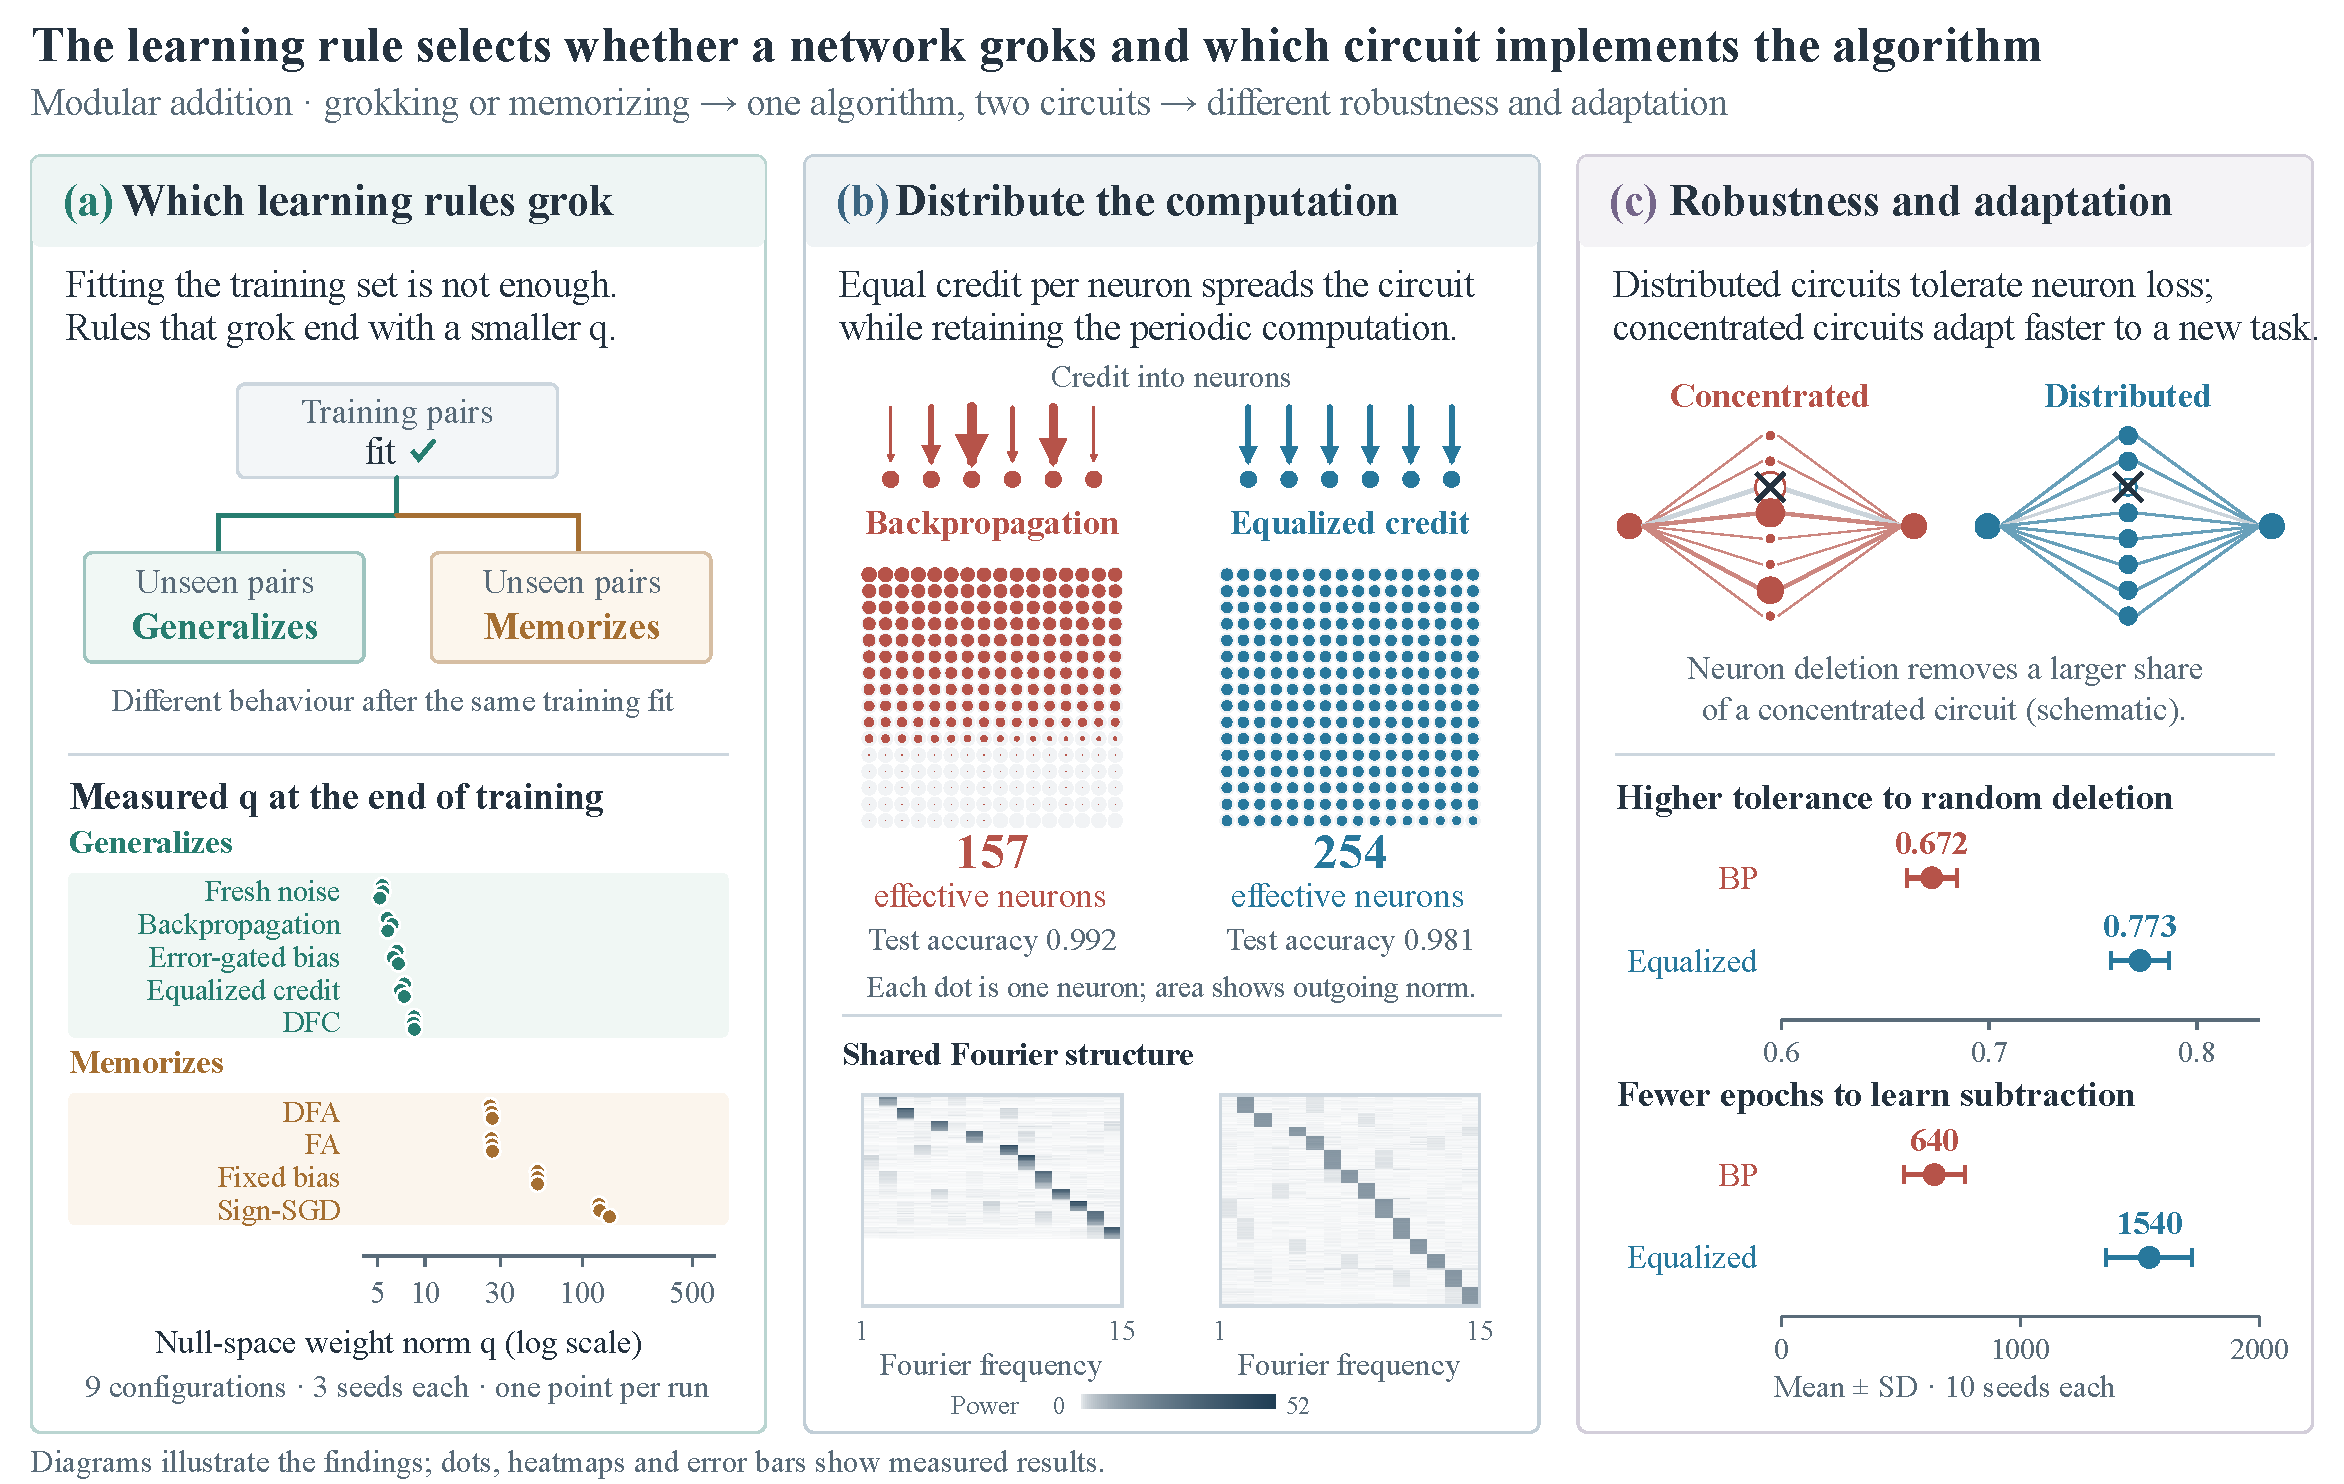
\includegraphics[width=\linewidth]{figures/fig1_hero.pdf}\end{center}\vspace{-3mm}
\caption{The learning rule decides whether the network groks and how many units carry the solution. \textbf{(a)} The first hidden layer of two networks differing only in how evenly the error signal is split across units: Fourier power per unit, darker for more power, beside each unit's outgoing weight norm, units grouped by dominant frequency, idle units last. Both compute the same periodic solution from a few frequencies and differ in how many units carry it, an effective $154$ of $256$ units with $84$ idle against an effective $254$ with none (Section~\ref{sec:select} defines the effective count, seed nearest the three seed mean, shared color scale). \textbf{(b)} Whether a rule groks is decided by whether its update dies out at the minima of the loss: each rule and control is placed by the size of its update's orthogonal part at the solution against how persistently that part keeps one direction. Only rules keeping both land in the shaded corner, and exactly those memorize, with DFA and layerwise FA so close that their two crosses overlap. Backpropagation and our rescaling control only rescale the gradient, so they cannot test the criterion. \textbf{(c)} How many units carry the solution, placed by which parameters share one normalizer in the rule's update. The mixed setting combines a layer statistic with a single weight statistic. Every other choice lands in the shaded band around backpropagation, and only rules acting one unit at a time leave it, Lion \citep{chen2023lion} most sharply, its update sizes uniform, its solution concentrated. \textbf{(d)} The position has a price: solutions spread over many units survive unit deletion better and adapt to a new task more slowly.}
\label{fig:main}
\end{figure}

All of that work treats the sparse circuit as the solution the task demands, yet every network behind it was trained with backpropagation, which is only one procedure for turning an error into weight updates (a \emph{learning rule}). What the rule contributes to the circuit has therefore never been separated from what the task requires, and this paper asks: \emph{how does the learning rule influence grokking?}

We answer by changing only the learning rule while holding everything else fixed, across tasks and architectures (Figure~\ref{fig:main}). Different rules give different circuits: at matched test accuracy, loss, weight norm and margin, the number of units carrying the computation runs from $154$ to $254$ out of $256$, and four rules do not grok at all. The reported sparsity \citep{power2022grokking,nanda2023progress,gromov2023grokking} is therefore a fact about backpropagation rather than about the task.

Two learning rules can differ in many things at once, so to test what a unit's share of the error signal, its \emph{credit}, does to the circuit, we must move it in isolation, with the optimizer and every update direction held fixed. We therefore construct a rescaling of per-unit credit that provably leaves the objective and every per-unit update direction unchanged, and rescaling credit this way spreads the circuit over more units. Published optimizers differ in how widely they share one normalization, so we apply the same rescaling over groups of units instead of single ones, and the same behaviour appears (Section~\ref{sec:law}). This leads to three findings:

\emph{Finding 1, direction. Whether a rule groks at all is decided by whether it comes to rest at the minima of the loss.} A rule whose update still pushes somewhere at those minima has different stationary points than the loss, so it cannot end where gradient descent ends. The push is measured by the part of the update orthogonal to the gradient, which we call the rule's \emph{transverse component}: if it fades as the loss falls the rule keeps gradient descent's minima and weight decay still drifts the network onto the low norm solution, and if it survives it displaces every one of those minima (Section~\ref{sec:direction}).

\emph{Finding 2, grain. Among the rules that grok, how many units carry the circuit is decided by how many parameters share one normalization, which we call a rule's \emph{grain}.} Only rules that give each unit its own normalizer, one shared by all the weights going into a neuron, spread the circuit. A finer grain, one single weight at a time, and a coarser one, a whole weight matrix at once, both leave the circuit where backpropagation puts it, however drastically the update is transformed (Section~\ref{sec:law}).

\emph{Finding 3, the price. The concentrated and the distributed end are not interchangeable.} Distributed circuits survive random and targeted deletion far better, concentrated ones adapt to a new task about twice as fast, and either end can be selected before or after grokking, so choosing a rule is choosing between these two properties. This holds across tasks (modular operations, the non-abelian group $S_5$, sparse parity) and architectures (multilayer perceptrons, a transformer), in Section~\ref{sec:fragile}.

We test twelve published rules, eight optimizers from LARS \citep{you2017lars} to Shampoo \citep{gupta2018shampoo} and four credit assignment algorithms including feedback alignment \citep{lillicrap2016feedback} and sign-SGD \citep{bernstein2018signsgd}. From the findings we predict where all twelve land, the optimizers from their grain and the algorithms from their transverse component, and every prediction holds (Tables~\ref{tab:twoaxis} and~\ref{tab:zoo}). We also analyze deep feedback control and demonstrate grokking for a control driven rule, to our knowledge the first.

\section{Background and related work}
\label{sec:background}

\subsection{Grokking and the assumed solution}
Grokking was first reported on algorithmic tasks and later beyond them \citep{power2022grokking,liu2022omnigrok}. For modular arithmetic, the circuit is known in detail as a Fourier computation \citep{nanda2023progress}, and the solution can be written in closed form \citep{gromov2023grokking}.

That characterization is mostly read as what the task demands, and the delayed generalization is then explained by the network drifting toward that one sparse solution \citep{varma2023circuit,liu2022omnigrok,kumar2024grokking}. Within the works that depart from the unique solution, most change the computation along with it. \citet{zhong2023clock} vary the architecture, hyperparameters or seed and get a qualitatively different algorithm. \citet{merrill2023tale} separate a sparse subnetwork that generalizes from a dense one that memorizes, so their two sides compute different things. The closest formal account of the grokked solution's structure bundles two properties, since \citet{morwani2024feature} prove that max-margin solutions of a one hidden layer model combine single frequency neurons with a computation carried by many units. \citet{luo2021phase} condense a two layer network onto few effective neurons by shrinking the initialization, and \citet{thilak2022slingshot} show adaptive optimizers change whether grokking happens, in both cases without asking which circuit forms. None of this work compares networks that compute the same algorithm over different numbers of units.

The strongest form of the task-fixes-the-solution reading is \emph{universality}, the claim that every network solving a task uncovers the same circuit, so that a circuit found in one network stands for the task itself \citep{chughtai2023toy}. The claim has two levels that current evidence does not separate: the computation, which frequencies are used and how they are composed, and the layout, how many units carry it. The first level is not contested here. Every network behind the results above was trained with backpropagation, so whether the task fixes both levels, or only the first, has never been asked, and that gap is what this paper addresses.

\subsection{Alternatives to backpropagation}
The results above were all obtained with backpropagation, but it is not the only way to turn an error into weight updates. Feedback alignment \citep{lillicrap2016feedback,nokland2016dfa}, predictive coding \citep{whittington2017pc}, equilibrium propagation \citep{scellier2017eqprop} and deep feedback control (DFC) with its least control principle \citep{meulemans2021dfc,meulemans2022lcp} each compute a different error signal, and each is asked the same question, whether it can match backpropagation's accuracy. What solutions they select is left open, and none of them has been run on a task whose circuit is understood. Two results come closest and still stop short: feedback alignment aligns early and then memorizes \citep{refinetti2021align}, and \citet{mallinar2025agop} reach grokking without backpropagation, but in a kernel method rather than a network, so there is no per unit circuit to read. The variation this paper needs therefore already exists in the literature, and nobody has pointed it at grokking, so nothing says whether a rule outside the gradient family can grok, or what circuit it builds when it does.

\subsection{The credit assignment algorithms and optimizers under test}
\label{sec:ruleset}
Training involves two procedures that this paper keeps apart. The procedure that computes each parameter's error signal is the \emph{credit assignment algorithm}, backpropagation being one example, and the signal a hidden unit receives is that unit's \emph{credit}. The procedure that turns those signals into the weight update, SGD or Adam, is the \emph{optimizer}, and the pair of the two is the \emph{learning rule}, rule for short. The split matters: the same credit can memorize under one optimizer and grok under another.

We select twelve rules to cover both parts and a broad spectrum within each, from optimizers in wide current use to algorithms that leave the gradient behind. Eight vary the optimizer and keep backpropagation's credit, differing in how many parameters share one normalizer. LARS \citep{you2017lars} rescales a whole layer by one scalar, Muon \citep{jordan2024muon} and Shampoo \citep{gupta2018shampoo} transform a whole weight matrix, RMSProp \citep{tieleman2012rmsprop}, Lion \citep{chen2023lion} and Adafactor \citep{shazeer2018adafactor} work on each single weight, LAMB \citep{you2020lamb} combines a layer statistic with a single weight statistic, and Nero \citep{liu2021nero} normalizes the incoming weights of one neuron. Four vary the credit assignment algorithm: feedback alignment from above, in its direct and layerwise forms \citep{nokland2016dfa,lillicrap2016feedback}, joined by sign-SGD \citep{bernstein2018signsgd} and K-FAC \citep{martens2015kfac}, all delivering near uniform credit magnitude, which makes them the probes for separating magnitude from direction. Predictive coding and equilibrium propagation stay out, since each needs its own inference loop and objective and could not be run at the matched setting the comparison requires. DFC completes the set as the furthest departure we can run at that setting, the one rule here whose credit is not a transformation of the gradient at all: it replaces the backward pass with a controller \citep{meulemans2021dfc} that drives the network toward a compromise between its own output and the label, and the controller exists only during training, so the trained network is architecturally identical to every other network here.

\section{Setup}
\label{sec:setup}

We study modular arithmetic. The network receives two operands $a, b \in \mathbb{Z}_p$ as concatenated one hot vectors and predicts $c = (a \circ b) \bmod p$ for an operation $\circ \in \{+, -, \times\}$, with addition the primary task. Our network is fully connected, with ReLU units, two hidden layers of width $n = 256$ and a linear readout, and it predicts the class with the largest \emph{logit}, the raw pre-softmax score. \citet{gromov2023grokking} and \citet{morwani2024feature} study this task with the same kind of model. We use prime moduli so that $\mathbb{Z}_p$ is a field with the Fourier structure the grokking literature studies, and sweep $p \in \{23,31,47,59\}$ with $p=31$ the default (Appendix~\ref{app:repro}). Training minimizes the cross entropy with weight decay $10^{-3}$ under Adam \citep{kingma2015adam}, shared by every rule unless stated otherwise (Appendix~\ref{app:consumer}), and hidden weights are initialized Kaiming normal \citep{he2015delving}. We say a run \emph{groks} when training accuracy reaches $1.0$ while test accuracy first exceeds $0.97$ only much later. Sections~\ref{sec:direction} to~\ref{sec:fragile} study modular addition at $p=31$ over three seeds unless stated otherwise.

\section{Whether a rule groks is decided at the minima of the loss}
\label{sec:direction}

\begin{table}[t]
\caption{The rules on both axes: backpropagation and the credit knob, our per unit rescaling of its credit magnitudes (Section~\ref{sec:select}), beside five of the twelve published rules (Table~\ref{tab:zoo} holds the rest). The Normalizes column gives which parameters share one normalizer in the rule's update, $\downarrow$ and $\uparrow$ the concentrated and the distributed end. Circuit PR and credit PR are the participation measures of Section~\ref{sec:select}, at $p=31$ over three seeds, standard deviations on circuit PR, credit PR a seed mean (Appendix~\ref{app:baselines}). A dash means not applicable: DFC and the feedback alignment rules do not rescale the gradient, a rule that builds no circuit has no circuit PR, and K-FAC here applies its own raw step (Appendix~\ref{app:consumer}).}
\label{tab:twoaxis}
\begin{center}
\scriptsize
\renewcommand{\arraystretch}{0.88}
\begin{tabular}{lccccl}
\toprule
Rule & Normalizes & Credit PR & Circuit PR & Test & Outcome \\
\midrule
LARS \citep{you2017lars} & per layer & $0.53$ & $0.63\,(0.04)$ $\downarrow$ & $0.970$ & groks \\
Backpropagation      & none           & $0.59$ & $0.60\,(0.02)$ $\downarrow$ & $0.996$ & groks \\
DFC                  & --- & $0.94$ & $0.92\,(0.00)$ $\uparrow$ & $1.000$ & groks \\
Knob ($\beta{=}0.25$)& per unit       & $0.96$ & $0.94\,(0.01)$ $\uparrow$ & $0.996$ & groks \\
Knob ($\beta{=}1$)   & per unit       & $1.00$ & $0.99\,(0.00)$ $\uparrow$ & $0.975$ & groks \\
\midrule
Sign-SGD             & per parameter  & $1.00$ & --- & $0.000$ & memorizes \\
K-FAC                & per unit       & $0.98$ & --- & $0.486$ & memorizes \\
DFA                  & ---            & $0.98$ & --- & $0.000$ & memorizes \\
FA (layerwise)       & ---            & $0.96$ & --- & $0.000$ & memorizes \\
\bottomrule
\end{tabular}
\end{center}
\end{table}

Changing the learning rule does not always preserve grokking. Backpropagation, DFC, the credit knob and all eight published optimizers grok, reaching test accuracy above $0.97$ (Table~\ref{tab:twoaxis}, with the optimizers in Table~\ref{tab:zoo}), while four rules never generalize at all and stay at chance on held out data however long they train. What separates the two groups is where training comes to rest. Once training accuracy reaches $1.0$, the parameters lie on $\mathcal{M} = \{\theta : L_{\mathrm{train}}(\theta) \approx 0\}$, the set of parameters that fit the training data, and stay inside it. We call it the \emph{interpolating set}. There the training loss is constant, so only the weight decay still pulls, and it pulls toward the solutions in $\mathcal{M}$ with the smallest weights. Those are the solutions that generalize, since memorizing needs larger weights than the periodic solution does \citep{liu2022omnigrok}.

Whether a rule comes to rest there is decided by the part of its update that is not the gradient. Split a rule's update into the gradient of the regularized loss and a remainder orthogonal to it, which we call the rule's \emph{transverse component} $\vb_t$. Training halts only where the full update vanishes, so a rule whose transverse component is nonzero at the minima of the loss cannot halt at one. It halts away from them, and the offset is largest along $\mathcal{M}$, where the loss is flattest and the circuit is decided, so training ends off the grokked circuit while training accuracy stays perfect (Proposition~\ref{prop:persist}, with the size of the offset in Appendix~\ref{app:theory}). Both parts shrink as training converges, so the size of $\vb_t$ on its own says little and we compare it against the gradient: the component \emph{survives} when the ratio $\|\vb_t\|/\|\vg_t\|$ does not fall as the loss does. This is the criterion we test: \emph{if a rule's transverse component vanishes as the loss falls, the network groks.}

For the rules that grok, the reason can be read from the update (Appendix~\ref{app:mech}). Backpropagation, LARS and the knob only rescale the gradient, so any orthogonal part they carry shrinks as the gradient does. DFC demonstrates that a rule can satisfy the criterion without staying close to the gradient: its update sits far from the gradient throughout training, and its transverse component still falls from $0.410$ of the gradient norm to $0.038$, because the controller signal driving it is proportional to the remaining output error, and training closes that error. A rule can therefore estimate the gradient badly and still grok, as long as the error fades where the loss does.

Each rule that fails to generalize holds a component that does not fade. Feedback alignment routes the error through a fixed random matrix, so its component keeps one direction and is still about a quarter of the gradient norm at the end. Sign-SGD's update has norm $\eta\sqrt{d}$ whatever the gradient, so at a fixed learning rate it cannot shrink relative to a vanishing gradient, and it still memorizes at every learning rate we swept, down to $10^{-5}$ (Appendix~\ref{app:named}). K-FAC fails for a different reason, and it shows that the credit assignment algorithm does not decide the outcome on its own: its own raw step memorizes, while the same credit handed to Adam groks (Appendix~\ref{app:consumer}). Whether a circuit forms is a property of the algorithm and the optimizer together, not of the credit alone.

The criterion holds without exception across these rules and three constructed controls, which also rule out three alternative explanations (Appendix~\ref{app:mech}). \emph{Persistence of direction} fails: DFC's transverse direction is almost as persistent as a fixed-bias control, autocorrelation $0.97$ against $0.99$, yet DFC groks and the control memorizes, and scaling that same control by the current loss so that it fades restores grokking everywhere it had destroyed it. \emph{Distance from the gradient} fails: at matched cosine, fresh noise leaves grokking intact down to $0.2$ while the fixed bias kills it by $0.7$. \emph{Credit magnitude} fails: the four rules that memorize spread credit \emph{more} evenly than backpropagation, and swapping feedback alignment's random matrix for the transpose of the forward weights recovers grokking, which validates our implementation. What selects a circuit is therefore not what decides whether one forms at all.

\section{The rules that grok share the algorithm but not the circuit}
\label{sec:select}

The rules that grok all reach the same test accuracy, and they all implement the same algorithm. What differs is the circuit, the way that algorithm is laid out across the units.

\subsection{Same algorithm, different circuits}
Comparing circuits needs a measure of how many units carry the computation. Indexing the $n$ units of a hidden layer by $j$ and writing $a_j = \|\mW^{\mathrm{out}}_{:,j}\|_2$ for unit $j$'s \emph{outgoing norm}, the norm of the weights carrying its output onward, the \emph{participation ratio} is
\begin{equation}
\mathrm{PR} \;=\; \frac{\big(\sum_j a_j\big)^2}{n \sum_j a_j^2} \;\in\; (0, 1],
\label{eq:pr}
\end{equation}
so $\mathrm{PR} = 1$ when every unit contributes equally, $\mathrm{PR} = 1/n$ when one unit does all the work, and $n \cdot \mathrm{PR}$ reads as an \emph{effective unit count} (Proposition~\ref{prop:pr}). Computed on the outgoing norms we call it \emph{circuit participation}. It does not depend on a choice of basis and does not move when the readout is rescaled (Appendix~\ref{app:pr}).

Backpropagation and DFC sit at opposite extremes. Backpropagation carries the computation on roughly $154$ of $256$ effective units ($n \cdot \mathrm{PR}$, Equation~\ref{eq:pr}), which we call a \emph{concentrated} circuit, and DFC on $254$, a \emph{distributed} one. The two are matched on test accuracy and on the mean gap between the correct logit and the largest incorrect one, which we call the \emph{logit margin}, so neither circuit simply fits the data better than the other (Table~\ref{tab:twoaxis}, Figure~\ref{fig:endpoints}).

The computation itself is the same. Both rules find the periodic Fourier algorithm that existing theory derives from the task and the architecture \citep{nanda2023progress,gromov2023grokking}: keeping only the strongest input frequencies recovers $95\%$ of accuracy for either, neither builds the alternative algorithm reported by \citet{zhong2023clock}, their pizza construction, and changing the rule costs no more functional agreement than changing the seed (Appendix~\ref{app:algo}). That DFC groks at all is, to our knowledge, the first demonstration of grokking under a control driven rule.

\subsection{The credit knob}
\label{sec:rules}
Backpropagation and DFC differ in many things at once, so the gap between $154$ units and $254$ does not yet show that the credit split caused it. We therefore set DFC aside and work inside backpropagation alone, changing how evenly its credit is spread across units and reading off the resulting circuit. Everything else is held fixed: the same network, data, initialization, optimizer, learning rate, loss, and weight decay of $10^{-3}$, a setting backpropagation needs to grok at all \citep{power2022grokking,nanda2023progress}. The optimizer and the learning rate are shared, so the weight decay acts the same way in every run, and a structural difference can come only from how credit reaches the weights. The instrument is the \emph{credit knob}, built to ablate the credit split rather than to imitate a published rule.

The knob interpolates backpropagation's per-unit credit toward uniform with strength $\beta \in [0,1]$. The gradient of a weight matrix has one row per unit of the layer it feeds, row $j$ holding the gradient of every weight going into unit $j$. Writing $\vg_j$ for that row, so that $\|\vg_j\|$ is the credit unit $j$ receives, and $\bar{g} = \frac{1}{n}\sum_l \|\vg_l\|$ for the mean row norm,
\begin{equation}
\vg_j \;\leftarrow\; \frac{\vg_j}{\|\vg_j\|} \Big( (1-\beta)\, \|\vg_j\| + \beta\,
\bar{g} \Big),
\label{eq:knob}
\end{equation}
which preserves every row's direction and changes only how magnitude is spread across units. It rescales the weights entering a hidden layer, one unit at a time, and those units are the ones circuit participation is read from, so credit and circuit describe one set of neurons from opposite sides. The effect stays where it is applied, since equalizing one layer redistributes that layer and leaves the others untouched (Appendix~\ref{app:imposed}), and the transformer runs apply the knob to every linear map (Appendix~\ref{app:transformer}). At $\beta = 0$ the knob is plain backpropagation, and at $\beta = 1$ every unit receives credit of equal magnitude. The rescaled update is a descent direction at every $\beta$ (Proposition~\ref{prop:descent}) and still minimizes backpropagation's cross entropy loss, so the two ends are loss matched by construction rather than by tuning, and Appendix~\ref{app:baselines} measures what alternative interventions change instead.
Since the knob changes no term of the objective, the set of minima is the same at every $\beta$ and only which of them the run ends in changes.

Equation~\ref{eq:pr} on the row norms $\|\vg_j\|$ says how evenly a rule spreads credit, the quantity a rule sets directly, and we call it \emph{credit participation}, credit PR beside circuit PR in tables. The two describe those neurons from either side: circuit participation reads their outgoing weights in the trained network, credit participation the incoming updates a rule delivers while it trains, taken after that rule's own rescaling and averaged over the last $800$ epochs. The vector of per-unit credit magnitudes $(\|\vg_j\|)_j$ is a rule's \emph{credit profile}.

\paragraph{The credit split decides how many units the circuit uses.} Turning the knob from $\beta=0$ to $\beta=1$ equalizes credit and drives circuit participation from $0.60$ to $0.99$ over ten seeds, past where DFC sits, at fixed loss, margin, norm and test accuracy (Figure~\ref{fig:steer}). Since nothing else varied, how evenly credit is split across units is what decides how many units carry the computation, and Proposition~\ref{prop:select} works the mechanism through in a model small enough to solve exactly. Two Fourier readouts rise with it: \emph{spectral entropy}, how widely the input weights' Fourier power \citep{nanda2023progress} is spread over frequencies, and \emph{per neuron periodicity}, the mean share of a unit's power on its strongest single frequency. Both are invariant to output scale and written out in Appendix~\ref{app:repro}. The knob is not simply breaking the network: both ends reach test accuracy above $0.97$, margins between $4.94$ and $5.16$ and training cross entropy $0.040$, so it selects among grokked solutions. Full equalization costs about two points of test accuracy, which $\beta=0.25$ avoids while still reaching a highly distributed circuit.

Credit and circuit are tightly coupled here: a unit's credit and its outgoing norm correlate at $0.995$ across units. A correlation that size does not say which of the two drives the other, and both could instead be tracking how much each unit matters to the task. We therefore remove, one at a time, three things the credit could be working through: the information in the profile, its persistence, meaning whether the same units keep receiving the same credit, and its timing, meaning when during training it acts (Appendix~\ref{app:imposed}). \emph{An imposed profile strips the information.} An artificial profile, drawn to a chosen participation and dealt to units at random, makes the circuit match its shape to a mean absolute deviation of $0.018$ across five targets, though it carries no information about any unit's role. \emph{A permuted profile strips the persistence.} Shuffling backpropagation's own magnitudes across units at every step destroys the concentration, landing at $0.992$, so a circuit concentrates only if credit focuses on the \emph{same} units over time. \emph{A switch after grokking strips the timing.} Turning the knob on only after backpropagation has grokked reorganizes the finished circuit from $0.61$ to $0.99$ within five thousand epochs at test accuracy $0.997$, and turning it off re-concentrates it, so the layout is a state the rule maintains rather than one locked in at the transition. Given the three interventions, the per-unit credit profile is sufficient to set the circuit's concentration. The gap between backpropagation and DFC is therefore a difference in credit, not two separate phenomena. Both ends hold their structure for $200{,}000$ epochs, ten times our standard budget, so they are two distinct solutions rather than one reached at two speeds (Appendix~\ref{app:long}).

\subsection{Grain is the mechanism, and it places published optimizers}
\label{sec:law}

The knob shows what per-unit credit does when we set it ourselves. Published optimizers rescale credit as well, each over its own group of parameters, and that group is what decides whether the circuit moves at all. The eight optimizers of Section~\ref{sec:ruleset} differ in which parameters share one normalizer, and we call that group of parameters the rule's \emph{grain}. The knob's grain is one unit, and to vary the grain directly we generalize Equation~\ref{eq:knob} at $\beta = 1$ to a partition of the $n$ rows into groups of $m$ units, rescaling all rows of a group by one common factor so that every group ends up with the same mean credit:
\begin{equation}
\vg_j \;\leftarrow\; \vg_j\, \frac{\bar{g}}{\bar{g}_{B(j)}},
\qquad
\bar{g}_{B(j)} \;=\; \frac{1}{m}\sum_{l \in B(j)} \|\vg_l\|,
\label{eq:grain}
\end{equation}
where $B(j)$ is the group containing unit $j$ and $\bar{g}$ is the overall mean row norm of Equation~\ref{eq:knob}. At $m = 1$ this is the knob at $\beta = 1$, and at $m = n$ it rescales the whole layer at once and changes nothing.

A single factor multiplies every unit in its group by the same amount, so it can shift credit from one group to another but cannot change how credit is divided \emph{within} a group. If one unit in a group starts with twice the credit of another, it keeps twice the credit after any common factor is applied. Uneven credit inside a group therefore survives any amount of equalizing, and it disappears only once each group holds a single unit. Proposition~\ref{prop:grain} derives the prediction that follows: circuit participation stays near backpropagation's value while groups hold several units, and reaches the distributed end only once every group holds one.

We test this by running Equation~\ref{eq:grain} at shrinking group sizes. From whole-layer groups down to eight units per group the circuit does not move: it stays within $0.023$ of the circuit participation backpropagation reaches when no credit is equalized at all, which we call \emph{plain flow}. It reorganizes only over the last three halvings, from eight units per group to four, two and one, and the same threshold appears at $p=31$, $p=47$, $p=59$ and on $S_5$ (Figure~\ref{fig:law}b plots circuit participation against group size). Proposition~\ref{prop:grain} predicts the whole curve to within $0.08$ from a single measurement at the whole-layer setting, with nothing else fitted (Appendix~\ref{app:grain}).

\begin{figure}[tb]
\vspace{-1mm}\begin{center}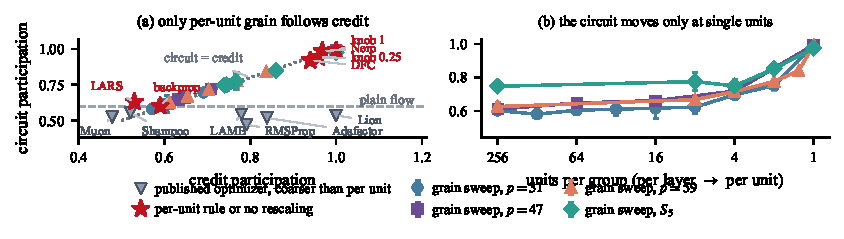
\includegraphics[width=0.82\linewidth]{figures/fig_law.pdf}\end{center}\vspace{-3mm}
\caption{Grain decides which of the two branches a rule falls into. Every marker is measured, every rule is labelled, and the two lines are the prediction, fitted to nothing: a per-unit rule, or one that rescales nothing, should land on circuit $=$ credit, its circuit as spread as its credit, and any other grain at plain flow, backpropagation's own $0.60$. \textbf{(a)} Circuit against credit participation for the grain sweep, equalizing credit across groups of units at $25$ settings on four tasks, with the named rules of Table~\ref{tab:twoaxis} (stars) and the six optimizers that normalize per parameter, per matrix or factored (triangles). \textbf{(b)} The same sweep against group size, where the circuit moves only once groups reach single units. Bars one standard deviation, three seeds.}
\label{fig:law}
\end{figure}

\paragraph{The grain law.} \emph{Only a rule that rescales credit one unit at a time can move the circuit at all. When it does, the circuit participation comes out equal to the credit participation, so even credit gives a distributed circuit and uneven credit a concentrated one. Any other grain leaves the circuit concentrated, whatever its credit looks like.} The law follows from Proposition~\ref{prop:grain}'s model and can be applied to a rule by inspecting its update equation, without training it. Backpropagation and the knob are the two cases already seen, one rescaling nothing and staying concentrated, the other rescaling per unit and following the credit it applies. DFC belongs with the knob, though we had to measure it rather than read it off an equation, since its credit is not a transformation of the gradient yet still reaches each unit separately. Across grain settings the mean gap between credit participation and circuit participation is $0.0074$ within a seed, the vertical distance from the circuit $=$ credit line in Figure~\ref{fig:law}a, while at every other grain the circuit ignores the credit and stays where plain flow would have left it.

The published optimizers are the second comparison: credit stays untouched and the whole optimizer is swapped, each rule at its own tuned learning rate. Weight decay is then not strictly comparable across rules, so we use these runs only to read off how many units each rule's circuit uses. RMSProp, LAMB, Adafactor, Lion, Muon and Shampoo all have grains other than one unit, so all six are predicted concentrated, and all six grok and land between $0.470$ and $0.555$ (Table~\ref{tab:zoo}, full scoring in Appendix~\ref{app:zoo}). LARS normalizes exactly as the knob does but per layer, and it stays concentrated too, at $0.613$. Nero is the set's one per-unit rule, so it alone is predicted distributed, and it lands there at $0.986$ (Appendix~\ref{app:named}). Lion is the sharpest test of the two. Its grain is per parameter, which predicts a concentrated circuit, and that is where it lands, at $0.535$. Its credit, on the other hand, is perfectly even, at credit participation $1.000$, because a sign update gives every row the same norm, so reading the credit alone would have placed it at the distributed end. Grain is the more accurate rule in general, not only here: predicting each rule from its credit fails four times in eight, where grain is right eight times in eight.

\section{The two ends trade robustness against adaptation speed}
\label{sec:fragile}

Section~\ref{sec:select} leaves a rule anywhere between a concentrated circuit and a distributed one, and neither position is free. Circuits spread over many units resist damage better, and concentrated ones can be repurposed for a new task faster. We define \emph{deletion tolerance} as mean test accuracy over nine damage levels in steps of $0.1$ from $0$ to $0.8$, each zeroing the outgoing weights of a random fraction of hidden units over $30$ masks, with \emph{targeted deletion} removing the highest norm units first and \emph{frequency removal} the same construction over input embedding Fourier components (Appendix~\ref{app:repro}), random del and targeted del in tables. Under random unit deletion \citep{averbeck2006population} the distributed circuits keep much more accuracy at the same damage, at shared loss, margin and norm, on every operation and modulus we run (Figure~\ref{fig:fragile}a, Appendix~\ref{app:figs}).

Proposition~\ref{prop:fluct} says why: deleting a fixed fraction of units removes, on average, the same fraction of every circuit's summed unit contributions, so what separates them is the fluctuation around that average, which falls as $1/\sqrt{n \cdot \mathrm{PR}}$. Two deterministic attacks rule out the alternative, that random deletion misses the concentrated circuit's weak points: deleting the highest norm units first widens the gap, and a greedy search on accuracy that never looks at norms needs $23$ of $256$ units to break backpropagation's circuit against $61$ for the knob's (Appendix~\ref{app:figs}, Table~\ref{tab:plane}). The spread itself does the work: forcing the outgoing norms to a chosen participation without touching the gradient reproduces the deletion tolerance to three decimals (Appendix~\ref{app:suff}).

Adaptation speed is the other side of the trade. It is read from training time rather than from outgoing norms, so it tests the same distinction without using the measure that defined it. We grok networks on addition at each $\beta$, then fine-tune on a second operation with plain backpropagation, so only the starting circuit differs. Adaptation time rises with $\beta$ at every step, from $640$ epochs at the concentrated end to $1540$ at the distributed one, with per seed ranges that do not overlap, and only the fully distributed start fails to beat the $1410$ epochs from scratch. Part of the reason is spare capacity, backpropagation's roughly $85$ of $256$ near idle units that a new task can claim without disturbing working structure, and Appendix~\ref{app:adapt} separates that from the rest. $\beta=0.25$ matches backpropagation's source accuracy within a point while still adapting half again as slowly. Neither end is better, and choosing a rule is choosing between the two properties.

\paragraph{The effect extends beyond grokking and Fourier circuits.}
Table~\ref{tab:scope} lists every setting we applied the knob in, each removing one thing the effect could have rested on, and none matters: the operation, the group structure ($S_5$, participation from $0.70$ to $0.97$), the presence of one agreed solution the literature has characterized (sparse parity, $0.15$ to $0.96$), and the architecture (a transformer block, $0.61$ to $0.99$), with test accuracy within one percentage point of backpropagation's throughout.

\section{Discussion and conclusion}

Universality survives at the level of the computation and fails at the level of the layout. Frequency ablation, the trigonometric fit and the run-to-run agreement all find the same periodic computation whichever rule trains, while participation and per neuron periodicity move with the rule. A claim about what a network computes is therefore safe, and a claim about how sparsely it does so holds only for the rule that produced it.

\paragraph{One solution set, two biases.} The parameter configurations realizing the grokked algorithm form a set rather than a point, and the direction and grain findings are statements about that set. Direction says which rules reach it, those whose transverse component vanishes there so their fixed points lie on it, and grain says where on it a rule stops, since normalizing one unit at a time biases a run toward the distributed end while every other grain leaves it at plain flow. Backpropagation and DFC sit at two extremes of one solution set, with the knob tracing the path between them. That makes credit assignment a practical \emph{implicit bias}, a preference among the solutions that fit, readable from an update equation without training the rule.

\paragraph{Limitations.} The direction criterion is stated for credit assignment algorithms that share one optimizer, since whether a circuit forms depends on the pair, and optimizers taken whole are covered by their own convergence analyses \citep{karimireddy2019errorfeedback,chen2024lion}. Grain predicts which rules reorganize the circuit rather than the exact participation the others settle at (Appendix~\ref{app:zoo}), and participation predicts damage resilience rather than how cleanly single neurons tune (Appendix~\ref{app:dissoc}). The knob spreads a circuit that starts concentrated, so on MNIST there is nothing for it to move, and the adaptation half of the trade-off needs a target task that can reuse the source. DFC is one controller rule rather than a survey of them, since it groks in a narrow window and underfits parity and $S_5$ (Appendix~\ref{app:dfcwindow}).

\paragraph{Reproducibility statement.} All experiments use small networks on algorithmic tasks (Section~\ref{sec:setup}, Appendix~\ref{app:repro}), and an anonymized repository with the scripts for every table and figure accompanies the submission.

\subsubsection*{AI use statement}

In this work, we used generative AI tools as coding assistants when implementing experiments and analysis scripts, to refine wording in text written by the authors, and to check the related work for completeness. The research ideas, the experimental design, the derivations and the conclusions are the authors' own. We have reviewed all AI-assisted work, reading and testing the code against the results it produces and checking every suggested reference and formulation. We take responsibility for the final content of this work, including text, claims or artifacts produced with the aid of generative AI.

\bibliography{iclr2027_conference}
\bibliographystyle{iclr2027_conference}

\appendix

\section{The grain sweep and the test on published optimizers}

\subsection{The grain sweep}
\label{app:grain}
The credit knob equalizes credit one unit at a time, and the sweep applies the same operation to \emph{groups} of units, which is what a normalizer of any coarser grain effectively does. We split the $n = 256$ units of the first hidden layer into $g$ equal groups of $m = n/g$ units, and at every step rescale each group's gradient rows by the single factor that brings its total credit to the average group's, leaving the split \emph{within} the group untouched. Sweeping $m$ from $256$ down to $1$ carries the rule from equalizing nothing to equalizing every unit separately, and Proposition~\ref{prop:grain} derives the participation each $m$ should produce.

Both ends check themselves. At $m = 256$ the rescaling is the identity, so this end must reproduce backpropagation, and it does, at $0.602\,(0.023)$ against the $0.60\,(0.02)$ measured elsewhere in the paper. At $m = 1$ it is exactly Equation~\ref{eq:knob} at $\beta = 1$, so this end must reproduce the knob, and it does, at $0.992$ against $0.99$. Only the grains between them carry new information.

The steep end carries most of the effect. Half of the total movement arrives in the last halving, from $0.753$ at two units per group to $0.992$ at one, and targeted deletion tolerance rises along the same curve, from $0.327$ to $0.576$. Groups of two are still groups: a rule that comes within a factor of two of the right grain gets almost none of the effect.

The same shape holds on $S_5$, flat through $0.749$ at four units per group and rising to $0.852$ and $0.974$, so the result stands on a non-abelian task where it cannot be an artifact of the Fourier structure of modular arithmetic. Two points inside the flat region sit below their coarser neighbour, by less than one standard deviation in both cases, so we read the region as flat rather than as non-monotone.

\subsection{The prediction on published optimizers}
\label{app:zoo}
Proposition~\ref{prop:grain} says that equalizing credit moves the circuit only when it is done one unit at a time, so knowing the level at which an optimizer normalizes should be enough to say where its circuit lands, without knowing anything else about how it works. We test that on eight published optimizers spanning five grains, per layer, per matrix, factored, per parameter and per neuron, and all eight land where their grain says (Table~\ref{tab:zoo}).

\begin{table}[!ht]
\caption{The grain prediction holds for all eight published rules, $8/8$ in the \emph{branch} column. Published rules chosen by grain (three seeds): LARS \citep{you2017lars}, RMSProp \citep{tieleman2012rmsprop}, LAMB \citep{you2020lamb}, Adafactor \citep{shazeer2018adafactor}, Lion \citep{chen2023lion}, Muon \citep{jordan2024muon}, Shampoo \citep{gupta2018shampoo} and Nero \citep{liu2021nero}. \emph{Branch} is what Proposition~\ref{prop:grain} predicts from the rule's grain alone, and $\checkmark$ marks it satisfied. The two anchor rows are the ends the sweep must reproduce by construction, so they carry no prediction. Seven rules grok here, and Nero reaches test $0.824$ at this learning rate and groks at its tuned rates, landing distributed in both runs (Table~\ref{tab:named}). Every rule of a grain other than per unit stays in the concentrated range whatever its credit participation does, and the per-unit rules land distributed.}
\label{tab:zoo}
\begin{center}
\footnotesize
\setlength{\tabcolsep}{4pt}
\begin{tabular}{llcccl}
\toprule
Rule & Grain & Test & Credit PR & Circuit PR & Branch \\
\midrule
Backpropagation & --- (anchor)  & $0.998$ & $0.586$ & $0.595$ & $0.60$ (anchor) \\
LARS            & per layer     & $0.967$ & $0.520$ & $0.613$ & plain flow $\checkmark$ \\
RMSProp         & per parameter & $0.992$ & $0.791$ & $0.470$ & plain flow $\checkmark$ \\
LAMB            & layer $\times$ param & $0.995$ & $0.779$ & $0.543$ & plain flow $\checkmark$ \\
Adafactor       & factored      & $0.991$ & $0.839$ & $0.518$ & plain flow $\checkmark$ \\
Lion            & per parameter & $0.985$ & $1.000$ & $0.535$ & plain flow $\checkmark$ \\
Muon            & per matrix    & $0.999$ & $0.478$ & $0.524$ & plain flow $\checkmark$ \\
Shampoo         & per matrix    & $0.986$ & $0.521$ & $0.555$ & plain flow $\checkmark$ \\
\midrule
Nero            & per neuron    & $0.824$ & $1.000$ & $0.960$ & tracks credit $\checkmark$ \\
Knob ($\beta{=}1$) & per unit   & $0.976$ & $1.000$ & $0.992$ & tracks credit (anchor) \\
\bottomrule
\end{tabular}
\end{center}
\end{table}

Optimization geometry is known to select among equally accurate interpolators, from steepest and mirror descent under different norms \citep{gunasekar2018implicit} to the $\ell_1$ bias of small initialization \citep{woodworth2020kernel}. Those results say \emph{that} the update selects. Ours says \emph{which statistic} does the selecting, the per-unit credit profile, and that its grain is decisive, since normalized methods grouping per layer or per parameter \citep{you2017lars,you2020lamb,bernstein2018signsgd} leave the circuit concentrated. This is complementary to rich versus lazy \citep{kumar2024grokking}, which varies the parameterization scale rather than how a fixed rule distributes credit.

\section{Implementation and reproducibility}
\label{app:repro}
\paragraph{Statistical reporting.} Every number is a mean over seeds with the standard deviation in parentheses, three seeds unless stated otherwise, with the same seeds across the rules being compared. With three to six seeds we quote $t$ intervals rather than bootstrap intervals. For the headline comparison the $95\%$ intervals do not overlap: participation $[0.535, 0.663]$ at $\beta=0$ against $[0.986, 0.998]$ at $\beta=1$, and deletion tolerance $[0.622, 0.720]$ against $[0.759, 0.819]$. The comparisons carrying the claims are powered, the $\beta$ endpoints, the grain sweep, adaptation on subtraction and the $S_5$ agreement between credit and circuit. The rest are reported as directional: LARS against backpropagation, where equality is the prediction, the two-block transformer, the two within-noise dips in the grain sweep, and addition to multiplication transfer. Deviations between applied and realized participation are computed within each seed and then averaged, since averaging first would let opposite errors cancel.

\paragraph{Circuit measures.} Write $\vu_j, \vv_j \in \R^p$ for the halves of hidden unit $j$'s input weight vector acting on the two operands, and $\hat{u}_j$ for the discrete Fourier transform of $\vu_j$. Unit $j$'s \emph{spectrum} is the power its input weights place on each frequency $k$, for $k = 1, \dots, \lfloor p/2 \rfloor$,
\begin{equation}
s_j(k) \;=\; |\hat{u}_j(k)|^2 + |\hat{v}_j(k)|^2,
\qquad
\hat{u}_j(k) = \textstyle\sum_{a=0}^{p-1} u_j[a]\, e^{-2\pi i k a / p}.
\label{eq:spectrum}
\end{equation}
Write $S(k)$ for the \emph{aggregate spectrum}, the sum of $s_j(k)$ over units normalized to total one. Spectral entropy is $-\sum_k S(k) \ln S(k) / \ln \lfloor p/2 \rfloor$, per neuron periodicity is $\frac{1}{n} \sum_j \max_k s_j(k) / \sum_k s_j(k)$, and the logit margin is $\gamma = \mathbb{E}[z_y - \max_{c \neq y} z_c]$, with $z$ the logit vector and $y$ the correct class. Credit participation is Equation~\ref{eq:pr} on the gradient rows $\|\vg_j\|$ of the layer a rule acts on, taken as the credit assignment algorithm hands them to the optimizer, so a rule's own rescaling, sign transform or trust ratio is already included while Adam's state is not, sampled every epoch over the last $800$ and averaged. It is read from a different set of parameters than circuit participation, so their agreement is not an identity of the measurement. Table~\ref{tab:baselines} reports the variant measured on Adam's effective step instead.

\paragraph{Networks and training.} Architecture and optimizer are those of Section~\ref{sec:setup}, with two details not stated there: training is full batch, with gradient norm clipping at $1.0$. The knob acts on the first hidden layer in the multilayer perceptron experiments, where deletion and circuit participation are measured on the same units, and the transformer runs apply it to every linear map (Appendix~\ref{app:transformer}). Seeds run from $0$, so a three seed number uses seeds $0$ to $2$, and runs use a single GPU. Every run is trained to convergence, far past its grokking transition and with participation no longer moving, which takes between $12{,}000$ and $70{,}000$ epochs depending on task, modulus and architecture, and Appendix~\ref{app:long} confirms the criterion by running ten times longer with nothing changing. Exact budgets and full configurations, with the scripts behind every table and figure, are in the anonymized repository accompanying the submission.

\paragraph{Deep feedback control.} With control error $\ve = \vy^* - \hat{\vy}$, the controller is leaky proportional integral and the control signal is injected into the layer dynamics,
\begin{align}
\vu_{\mathrm{int}} &\leftarrow \vu_{\mathrm{int}} + \mathrm{dt}\,(\ve - \alpha \vu),
\qquad \vu = \vu_{\mathrm{int}} + k_p \ve, \label{eq:controller}\\
\vv_i &\leftarrow \vv_i + \tau ( \mW_i \vr_{i-1} + \vb_i + \mJ_i^\top \vu - \vv_i ),
\qquad \vr_i = \phi(\vv_i), \label{eq:dynamics}
\end{align}
where $\mJ_i$ is the Jacobian from layer $i$ to the output along the current state. The controller of Equation~\ref{eq:controller} uses integration step $\mathrm{dt}=0.02$, time constant ratio $0.2$ (so $\tau = \mathrm{dt}/0.2$), proportional gain $k_p = 2.0$, leak $\alpha = 1.7\times 10^{-3}$, at most $500$ controller iterations, and convergence when the control signal change falls below $10^{-4}$. The control strength is $\lambda = 0.3$ for modular arithmetic and $0.5$ for parity. The feedback pathway delivers the control signal through the transpose Jacobian, following the reference implementation of \citet{meulemans2021dfc}. At equilibrium each layer then applies the local update
\begin{equation}
\Delta \mW_i \;\propto\; (\vr_i - \vr_i^{\mathrm{ff}})\, \vr_{i-1}^\top,
\label{eq:update}
\end{equation}
the product of the layer's own teaching signal, its controlled activity minus its feedforward activity, and its presynaptic activity.

\paragraph{Loss choices.} Backpropagation with an MSE to one hot target and weight decay collapses to the trivial constant predictor (test accuracy at chance, near zero weight norm), because weight decay dominates the small regression gradient. We therefore use cross entropy for the knob and all backpropagation baselines. DFC is target driven and does not have this failure mode.

\paragraph{Data fractions, and why the scaling analysis excludes $p=23$.} We train on a fixed fraction of the $p^2$ pairs, $0.60$ for addition and $0.58$ for subtraction and multiplication, with multiplication's absorbing pairs ($a=0$ or $b=0$) included identically for every rule. At $p=23$ that leaves $317$ examples over $23$ classes, and backpropagation does not reach the ceiling there at any budget we tried, $0.83$ to $0.93$ test at three times the standard budget, while DFC reaches $1.000$. The frequency count scaling of Appendix~\ref{app:figs} therefore rests on $p=31$, $47$ and $59$, and $p=23$ appears only where the partially grokked baseline is marked as such.

\section{Interventions that separate credit from the gradient}
Section~\ref{sec:law} shows that the circuit a rule builds matches the credit it applies. That match invites one objection: a unit's incoming gradient norm is proportional to its outgoing weight norm times its backpropagated error, so credit and circuit are coupled by arithmetic, and their agreement could be forced rather than causal. This section breaks the coupling from three sides, varying the rule, then the credit, then the weights.

\subsection{Published per-unit rules and a weight geometry control}
\label{app:named}

Nero \citep{liu2021nero} normalizes the update per neuron, which is the per-unit grain, so the theory says it must land distributed. It does, at two learning rates (Table~\ref{tab:named}), and its tolerance to targeted deletion, $0.626$, is the highest of any rule we measure.

If the knob worked only by keeping the input rows at equal norm, the result would be a fact about weight shape rather than credit. Forcing each row to a fixed norm after every step, with no rescaling of the gradient, leaves the circuit near backpropagation, at participation $0.661\,(0.015)$ against $0.595\,(0.023)$, with lower deletion tolerance (Table~\ref{tab:named}). Equal row norms alone do not do what the credit rescaling does. Weight normalization \citep{salimans2016weightnorm} extends that control to a published method. It reparameterizes each unit's incoming vector as one learned scale times a direction, a per-unit constraint on the weights that rescales no credit, and under plain backpropagation, with weight decay on the per-unit scales, it groks to test $0.993$ and stays concentrated at participation $0.466\,(0.026)$ over three seeds. A ubiquitous per-unit reparameterization of the weights lands with the row-norm control and not with Nero, which is the dissociation between weight geometry and credit at publication scale.

The sign-SGD sweep guards a boundary rather than the coupling: Table~\ref{tab:twoaxis} uses sign-SGD as the case of uniform credit that still memorizes, which only holds if the failure is not a tuning artifact. At learning rates $10^{-4}$ and $10^{-5}$ and at weight decay $10^{-2}$, it reaches test $0.000$ in every case while delivering credit participation $1.000$, so it is not. The failure also survives gating: multiplying the sign update by the current loss, so the step vanishes as the fit is reached, still memorizes at every learning rate from $10^{-4}$ to $10^{-2}$ over three seeds, which keeps the sign family scored by its convergence theory rather than by the fixed point case of Proposition~\ref{prop:persist}.

\subsection{Imposed credit profiles}
\label{app:imposed}
Imposed profiles are the direct test of the coupling objection, since the credit is supplied from outside the gradient and nothing the network computes can feed back into it. At every step we replace the per-unit magnitudes of the input layer update with a profile drawn to a chosen participation, keeping each row's direction and the summed norm, and dealing the profile to units at random so it carries no information about any unit's role. The grokked circuit follows the imposed value across the sweep, and deletion tolerance follows with it, at test accuracy above $0.96$ everywhere (Table~\ref{tab:named}). A profile uncorrelated with the gradient leaves no coupling to explain the match. Participation is a quantity we can set, and the circuit obeys it.

The last row is the sharpest test. It keeps backpropagation's own credit magnitudes and only changes who receives them, dealing them out in a fresh random order every step. The set of magnitudes is unchanged, so participation is identical at every step, and only persistence is destroyed: the unit receiving the largest share now is not the one receiving it next. That alone moves the circuit to $0.992$ against backpropagation's $0.613$. A concentrated circuit needs credit that concentrates on the \emph{same} units over time, since concentration that moves around averages away.

Two boundary notes. Concentrating credit does not undo a circuit that is already distributed: rescaling DFC's magnitudes away from uniform drives credit participation from $0.92$ to $0.31$ and per-neuron periodicity from $0.89$ to $0.33$, while test accuracy and the frequency spread stay put, so per-neuron structure follows the credit applied now and frequency coverage, once built, persists. And nothing here depends on initialization scale: across scales of $0.5$ to $4$, backpropagation stays between $0.586$ and $0.613$, the knob between $0.990$ and $0.998$, and applied credit tracks the grokked circuit to a mean absolute deviation of $0.008$ throughout.

The knob is also local to the layer it acts on. Applied to the second hidden layer instead of the first, that layer's circuit distributes to $1.000$ while the first layer's stays at plain flow, $0.593\,(0.004)$ with $86$ units idle, and applied to both layers it distributes both, at test accuracy $0.98$ and above throughout (three seeds). Each layer's circuit follows its own units' credit, so the agreement between credit and circuit is not one layer's norms dragging another's along.

\begin{table}[!ht]
\caption{Nero lands at the distributed end as its per-neuron grain predicts, equal row norms without credit rescaling stay near backpropagation, and the grokked circuit follows an imposed credit profile to a mean absolute deviation of $0.018$ even though the profile carries no information about any unit's role. Interventions that vary the rule and interventions that vary the credit ($p=31$, three seeds, standard deviations in parentheses, "no" meaning the rule does not grok). In the upper block the row-norm constraint keeps row norms equal without rescaling credit, and sign-SGD fails at every setting swept. In the lower block each profile is drawn to the target participation and assigned to units at random, and the last row keeps backpropagation's own magnitudes and permutes which unit receives which at every step. Each block has its own backpropagation run.}
\label{tab:named}
\begin{center}
\small
\setlength{\tabcolsep}{4pt}
\begin{tabular}{lccccc}
\toprule
Rule or condition & Test & Credit PR & Circuit PR & Random del & Targeted del \\
\midrule
\multicolumn{6}{l}{\emph{Varying the rule}} \\
Backpropagation & $0.998$ & $0.586$ & $0.595\,(0.023)$ & $0.672$ & $0.311$ \\
Nero \citep{liu2021nero} & $0.985$ & $0.968$ & $0.986\,(0.002)$ & $0.748$ & $0.626$ \\
Nero, lr $3\times10^{-3}$ & $0.978$ & $0.959$ & $0.983\,(0.001)$ & $0.728$ & $0.541$ \\
Row-norm constraint & $0.954$ & $0.611$ & $0.661\,(0.015)$ & $0.607$ & $0.256$ \\
Sign-SGD, lr $10^{-4}$ & $0.000$ & $1.000$ & no & --- & --- \\
Sign-SGD, lr $10^{-5}$ & $0.000$ & $1.000$ & no & --- & --- \\
Sign-SGD, lr $10^{-5}$, wd $10^{-2}$ & $0.000$ & $1.000$ & no & --- & --- \\
\midrule
\multicolumn{6}{l}{\emph{Varying the credit}} \\
Backpropagation & $0.997$ & $0.604$ & $0.613\,(0.016)$ & $0.673$ & $0.298$ \\
Imposed $0.60$ & $0.980$ & $0.600$ & $0.637\,(0.003)$ & $0.607$ & $0.240$ \\
Imposed $0.70$ & $0.981$ & $0.700$ & $0.727\,(0.001)$ & $0.663$ & $0.319$ \\
Imposed $0.80$ & $0.972$ & $0.800$ & $0.815\,(0.005)$ & $0.693$ & $0.420$ \\
Imposed $0.90$ & $0.969$ & $0.900$ & $0.902\,(0.005)$ & $0.723$ & $0.533$ \\
Imposed $1.00$ & $0.975$ & $1.000$ & $0.990\,(0.003)$ & $0.775$ & $0.599$ \\
\midrule
Reshuffled each step & $0.974$ & $0.979$ & $0.992\,(0.002)$ & $0.775$ & $0.601$ \\
\bottomrule
\end{tabular}
\end{center}
\end{table}

\subsection{Participation as a sufficient statistic}
\label{app:suff}
The knob reaches its participation by rescaling credit. A second route reaches the same participation without touching the gradient: constrain the outgoing norms of the first hidden layer to a chosen profile after every step. Comparing the two at matched participation asks which consequences follow from participation itself and which need the credit rescaling (Table~\ref{tab:suff}).

\paragraph{Deletion tolerance follows participation alone.} Proposition~\ref{prop:fluct} says it should, and at participation $0.99$ the two routes both reach random deletion tolerance $0.777$, matching to three decimals. That measure is computed from the norms we matched on, so we also ran the one attack that never consults a norm, the greedy search for the smallest set of units whose deletion drops test below $0.5$. It needs $66.7\,(11.1)$ units against the knob and $68.7\,(10.8)$ against the constraint, the same within seed spread. Targeted deletion, by contrast, is not comparable here: the constrained profile at $0.99$ is exactly uniform, so the attack has no highest norm unit to remove and degenerates to random deletion, which is why the $0.747$ in the table cannot be compared with the knob's $0.590$.

\paragraph{Adaptation time mostly follows it too.} At matched participation the constrained network takes $1480$ epochs against the knob's $1608$, and within the constrained family adaptation rises with participation, $740$, $1228$ and $1480$ epochs at $0.60$, $0.80$ and $0.99$. The remainder is spare capacity: at participation $0.60$ backpropagation keeps $87$ free units and adapts in $464$ epochs where the constrained network, with none, takes $740$, the split Appendix~\ref{app:adapt} details.

\paragraph{Per-neuron periodicity does not follow it.} The constrained family is flat, $0.865$ to $0.880$ from participation $0.60$ to $0.99$, while backpropagation at the same $0.60$ sits at $0.667$. Two networks with identical participation differ in per-neuron structure by about $0.20$, so periodicity is not a function of participation, and its agreement with the knob at $0.99$ is only both ends being high. This bounds the claim: participation is close to sufficient for the damage and adaptation consequences, and not for how cleanly single units tune.

\begin{table}[!ht]
\caption{Matching participation by constraining outgoing norms reproduces the deletion tolerance, so participation carries that consequence. The constraint route to the same participation (modular addition, $p=31$, five seeds, standard deviations in parentheses). Adaptation is epochs to test $0.9$ on subtraction, measured in this five seed run, so the backpropagation and knob values differ from the ten seed numbers of Table~\ref{tab:adapt}. The targeted deletion column for the constrained rows is an artifact of the exactly uniform profile, as explained above.}
\label{tab:suff}
\begin{center}
\footnotesize
\setlength{\tabcolsep}{4pt}
\begin{tabular}{lcccccc}
\toprule
Condition & Test & Circuit PR & Random del & Targeted del & Periodicity & Adapt \\
\midrule
Backprop             & $0.995\,(0.007)$ & $0.597\,(0.020)$ & $0.669$ & $0.321$ & $0.667$ & $464$ \\
Knob ($\beta{=}1$)   & $0.976\,(0.015)$ & $0.993\,(0.002)$ & $0.777$ & $0.590$ & $0.884$ & $1608$ \\
\midrule
Constrained $0.60$   & $0.987\,(0.016)$ & $0.600\,(0.000)$ & $0.647$ & $0.357$ & $0.865$ & $740$ \\
Constrained $0.80$   & $0.977\,(0.008)$ & $0.800\,(0.000)$ & $0.675$ & $0.449$ & $0.872$ & $1228$ \\
Constrained $0.99$   & $0.976\,(0.012)$ & $0.990\,(0.000)$ & $0.777$ & $0.747$ & $0.880$ & $1480$ \\
\bottomrule
\end{tabular}
\end{center}
\end{table}

\section{Controls and alternative explanations}
Each part of this section closes one alternative reading of the results.

\subsection{Matched cosine controls on credit direction}
\label{app:mech}
Two simpler explanations of DFC's distributed circuit come before ours, and both are wrong. The first is that DFC is backpropagation with a hidden penalty attached, reaching the gradient by another route. It is not: throughout training its update points about $66$ degrees off the true gradient, a cosine of $0.4$ rather than $1$. Cosine is how we report misalignment below, with $1$ along the true gradient and $0$ at right angles.

The second is that misalignment of that size is itself what distributes a circuit. Two matched-cosine controls settle it (Table~\ref{tab:direction}). Both force backpropagation's update to a fixed cosine with the true gradient, and they differ only in whether the transverse part is redrawn each step. Redrawn, transverse components in random directions cancel and grokking survives to cosine $0.2$. Held fixed, grokking is gone by cosine $0.7$, and by $0.4$ the network memorizes at feedback alignment's own per-neuron periodicity. The size of the misalignment is not what decides.

Consistency comes closer and is still not the answer, and DFC is what rules it out. We measure persistence by removing the update's projection onto the true gradient and correlating the remaining direction with itself $4000$ epochs later, so $1$ means one direction held. DFC's component is as persistent as the fixed bias control, $0.97$ against $0.99$, and it groks where the control memorizes. Nor does any scalar alignment number order the rules. Measured at the input embedding alone, K-FAC sits at cosine $0.98$ and memorizes, while DFC sits at $0.72$, below the $0.78$ at which feedback alignment memorizes, and groks.

What separates DFC is that its push is tied to its own error: the controller signal shrinks as the output reaches the target, so at the solution there is nothing left to push with, where a fixed bias never shrinks. The error-gated control isolates exactly that. Both arms apply one fixed bias per seed at the same initial cosine, and the gated arm additionally scales the transverse part by the current loss, fading it to $0.011$ of its initial size while its direction never changes. The constant arm groks $0/3$ at every cosine below $1$, and the gated arm $3/3$, at test $0.984$ to $0.995$. Fading a push that would otherwise destroy grokking restores it completely, which is what Proposition~\ref{prop:persist} requires.

\begin{table}[!ht]
\caption{Persistent misalignment, not misalignment itself, is what destroys grokking. Three matched-cosine controls on credit direction (modular addition, $p=31$, three seeds), all forcing the update to a fixed cosine with the true gradient at matched magnitude. Fresh noise is redrawn each step, the persistent bias holds one direction, and the error-gated arm holds the same direction scaled by the current loss, so it vanishes at the solution. DFC operates near cosine $0.4$ with an error-gated residual, and groks.}
\label{tab:direction}
\begin{center}
\small
\begin{tabular}{lccccc}
\toprule
Cosine to gradient & $1.0$ & $0.7$ & $0.5$ & $0.4$ & $0.2$ \\
\midrule
i.i.d.\ noise: grok rate       & $3/3$ & $3/3$ & $3/3$ & $3/3$ & $3/3$ \\
i.i.d.\ noise: spectral entropy & $0.85$ & $0.83$ & $0.85$ & $0.85$ & $0.84$ \\
i.i.d.\ noise: per-neuron      & $0.64$ & $0.57$ & $0.56$ & $0.56$ & $0.54$ \\
\midrule
persistent bias: grok rate     & $3/3$ & $0/3$ & $0/3$ & $0/3$ & $0/3$ \\
persistent bias: test          & $0.998$ & $0.607$ & --- & $0.000$ & $0.000$ \\
persistent bias: per-neuron    & $0.64$ & $0.44$ & $0.26$ & $0.23$ & $0.22$ \\
\midrule
error-gated bias: grok rate    & $3/3$ & $3/3$ & --- & $3/3$ & $3/3$ \\
error-gated bias: test         & $0.998$ & $0.984$ & --- & $0.995$ & $0.991$ \\
error-gated bias: per-neuron   & $0.63$ & $0.78$ & --- & $0.77$ & $0.75$ \\
\bottomrule
\end{tabular}
\end{center}
\end{table}

\paragraph{The criterion measured on trained rules.} The controls impose the criterion, and this measurement reads it off the rules as trained. At checkpoints through training we compare each rule's applied update $\vu$ with the true gradient $\vg$ at the same parameters, recording the transverse part $\vu_\perp$ in units of $\|\vg\|$ and the autocorrelation of its direction (Table~\ref{tab:survival}). Backpropagation and the knob are excluded by construction, since a positive reweighting's transverse part vanishes wherever the gradient does and Proposition~\ref{prop:persist}(i) cannot displace its critical points. The exclusion is itself a prediction, that every positive reweighting groks, which the knob, LARS and Nero all do, and the sign rules are scored by their convergence theory instead (Appendix~\ref{app:theory}).

\begin{table}[!ht]
\caption{Rules that memorize keep their transverse component at the solution, while DFC collapses its own and groks. The transverse component of each rule's update, measured against the true gradient at the same parameters (modular addition, $p=31$, three seeds). Early and late are the first and last quarter of checkpoints, late/early the ratio of the raw $\|\vu_\perp\|$, and \emph{survives} means a component of held direction is still there at the solution, the memorizing outcome. Backpropagation and the knob are excluded as positive reweightings.}
\label{tab:survival}
\begin{center}
\small
\begin{tabular}{lcccccc}
\toprule
Rule & Test & $\|\vu_\perp\|/\|\vg\|$ early & late & Late/early & Direction lag & Survives \\
\midrule
Backpropagation & $0.996$ & $0.000$ & $0.000$ & --- & $0.03$ & excluded \\
Knob ($\beta{=}1$) & $0.976$ & $0.132$ & $0.090$ & $0.57$ & $0.57$ & excluded \\
\midrule
Fixed bias & $0.000$ & $0.917$ & $0.917$ & $0.87$ & $0.99$ & yes \\
DFA & $0.000$ & $0.344$ & $0.234$ & $0.61$ & $0.94$ & yes \\
FA (layerwise) & $0.000$ & $0.340$ & $0.235$ & $0.60$ & $0.92$ & yes \\
\midrule
Fresh noise & $0.986$ & $0.917$ & $0.917$ & $0.77$ & $-0.00$ & no \\
Error gated bias & $0.995$ & $0.092$ & $0.026$ & $0.07$ & $0.99$ & no \\
DFC & $1.000$ & $0.410$ & $0.038$ & $0.16$ & $0.74$ & no \\
\bottomrule
\end{tabular}
\end{center}
\end{table}

Among the rules it covers the separation is complete: every rule that memorizes keeps a transverse component of substantial size whose direction persists at $0.92$ or above, and every rule that groks fails that description. A component destroys the circuit only when it keeps both its size at the solution and one direction. DFC keeps the direction, persistent at $0.74$, and loses the size, falling by a factor of eleven as the controller signal vanishes. Fresh noise keeps the size and holds no direction. Both grok, which places DFC with the tolerated cases rather than with the fixed bias it otherwise resembles.

\subsection{The same credit under two optimizers}
\label{app:consumer}
Everything above compares rules that hand their credit to one shared optimizer. Damped Gauss-Newton and K-FAC instead apply their own step, and both precondition the gradient by curvature. Both are positive definite reweightings, so their update vanishes wherever the gradient does, and Proposition~\ref{prop:persist}(i) therefore cannot displace their solutions however far from the gradient they point.

Applied with a raw step both memorize, and consumed by the same optimizer every other rule in the paper uses both grok (Table~\ref{tab:consumer}). The credit is identical in each pair and only the optimizer that applies it differs, so the failure was never a property of the credit, which is why K-FAC appears in the bottom block of Table~\ref{tab:twoaxis} with the configuration it was tested at rather than as a rule that cannot grok. Where they grok, their circuits also land by grain: Gauss-Newton stays concentrated at participation $0.540$ to $0.619$ across dampings, and K-FAC, the one rule of the pair that whitens per unit, lands at $0.790$, outside the concentrated range of every coarse grained rule we ran. The composition also runs the other way: handing the knob's equalized credit to Lion instead of the shared optimizer still lands distributed, at circuit participation $0.984\,(0.003)$ and test $0.974\,(0.010)$ over three seeds, where Lion on its own credit sits concentrated near $0.5$, so the per-unit rescaling travels with the credit whoever consumes it.

The same dependence shows up in the fragility we report elsewhere: DFC's narrow window (Appendix~\ref{app:dfcwindow}) and sign-SGD's sensitivity to its learning rate are the same phenomenon, a transverse component that is small enough at one operating point and not at another.

\begin{table}[!ht]
\caption{The same credit under two optimizers gives opposite outcomes, for both curvature rules. Test accuracy on modular addition ($p=31$, three seeds). A raw step is the rule applying its own update directly, and the shared optimizer is the one every other rule in the paper uses. Damping is the term added to the curvature matrix before inversion.}
\label{tab:consumer}
\begin{center}
\small
\begin{tabular}{llcc}
\toprule
Rule & Damping & Raw step & Shared optimizer \\
\midrule
Gauss-Newton & $10^{-2}$ & $0.000$ & $0.990$ \\
             & $10^{-1}$ & $0.000$ & $0.994$ \\
             & $1$       & ---     & $0.998$ \\
\midrule
K-FAC        & $10^{-1}$ & $0.001$ & $1.000$ \\
\bottomrule
\end{tabular}
\end{center}
\end{table}

\subsection{Optimizer and regularizer baselines}
\label{app:baselines}
Three familiar mechanisms could in principle produce a distributed circuit: an adaptive optimizer's preconditioning, ordinary regularization, and hyperparameter tuning. None of them produces ours (Table~\ref{tab:baselines}).

Adam equalizes per parameter, not per unit, so it neither produces this effect nor cancels it. Rerunning the sweep under plain SGD with momentum reproduces both endpoints, concentrated at $\beta=0$ (participation $0.53$, deletion tolerance $0.60$) and distributed at $\beta=1$ ($0.99$, $0.76$), and Adam's own effective per-unit credit, the participation of $m/\sqrt{v}$, reaches only $0.66$ at $\beta=0$ against the raw gradient's $0.59$ and $0.99$ at $\beta=1$, so it passes the knob's equalization through rather than supplying or absorbing it. Dropout does reach a distributed circuit, participation up to $0.99$, which is expected since it is a redundancy pressure, but it gets there by changing the objective, its solution drifting to higher margin ($5.3 \to 6.8$) and weight norm ($26.8 \to 30.2$) as the rate grows. Several routes lead to a distributed circuit, and the credit rescaling is the one that reaches it at backpropagation's own loss, margin and weight norm, changing nothing about the problem being solved.

Backpropagation cannot reach the distributed end at any setting of its own hyperparameters either. Sweeping three learning rates crossed with three weight decays, six of the nine grok and all six land concentrated, spanning only $0.530\,(0.008)$ to $0.626\,(0.012)$, short of even the midpoint between the two ends (Table~\ref{tab:bpgrid}). The three failures are at the highest weight decay, where test accuracy falls to $0.21$ to $0.36$, and a memorizing network's participation is not a grokked circuit. The grid also reproduces the agreement between credit and circuit six more times, with credit from $0.523$ to $0.613$ predicting circuit participation to a mean absolute deviation of $0.009$. The knob settings between the two ends fill the curve monotonically, $\beta=0.5$ at credit $0.99$ and circuit $0.98\,(0.00)$ with test $0.985$, and $\beta=0.75$ at $1.00$ and $0.99\,(0.01)$ with test $0.977$.

\begin{table}[!ht]
\caption{The credit-magnitude endpoint is not an Adam or dropout artifact ($p=31$,
three seeds). SGD+momentum reproduces the $\beta$ endpoints, Adam's effective per-unit credit stays concentrated, and dropout reaches a distributed circuit only by raising the margin and norm, which the knob does not.}
\label{tab:baselines}
\begin{center}
\small
\begin{tabular}{lccccc}
\toprule
Setting & Circuit PR & Random del & Margin & Norm & Note \\
\midrule
SGD+mom, $\beta{=}0$ & $0.53$ & $0.60$ & --- & --- & concentrated \\
SGD+mom, $\beta{=}1$ & $0.99$ & $0.76$ & --- & --- & distributed (as Adam) \\
Adam raw grad ($\beta{=}0$) & $0.59$ & --- & --- & --- & credit participation \\
Adam effective ($\beta{=}0$) & $0.66$ & --- & --- & --- & $m/\sqrt{v}$ credit participation \\
Adam effective ($\beta{=}1$) & $0.99$ & --- & --- & --- & Adam propagates the knob \\
LARS (per layer) & $0.63$ & $0.67$ & --- & --- & groks, stays concentrated \\
Dropout $0.1$ & $0.95$ & $0.79$ & $5.3$ & $26.8$ & objective changed \\
Dropout $0.5$ & $0.99$ & $0.82$ & $6.8$ & $30.2$ & objective changed \\
Credit knob $\beta{=}1$ & $0.99$ & $0.77$ & $5.2$ & $26.6$ & objective preserved \\
\bottomrule
\end{tabular}
\end{center}
\end{table}

\begin{table}[!ht]
\caption{Every setting that groks lands concentrated, and the applied credit tracks the grokked circuit throughout. Backpropagation under its own tuning ($p=31$, three seeds, standard deviations in parentheses). The three highest weight decay settings memorize, so their participation does not describe a grokked circuit.}
\label{tab:bpgrid}
\begin{center}
\small
\begin{tabular}{lccccc}
\toprule
Learning rate & Weight decay & Test & Credit PR & Circuit PR & Groks \\
\midrule
$3\times10^{-4}$ & $10^{-3}$        & $0.998$ & $0.613$ & $0.626\,(0.012)$ & yes \\
$3\times10^{-4}$ & $3\times10^{-3}$ & $0.983$ & $0.560$ & $0.571\,(0.027)$ & yes \\
$10^{-3}$        & $10^{-3}$        & $0.997$ & $0.604$ & $0.613\,(0.016)$ & yes \\
$10^{-3}$        & $3\times10^{-3}$ & $0.993$ & $0.523$ & $0.530\,(0.008)$ & yes \\
$3\times10^{-3}$ & $10^{-3}$        & $0.993$ & $0.589$ & $0.594\,(0.024)$ & yes \\
$3\times10^{-3}$ & $3\times10^{-3}$ & $0.988$ & $0.546$ & $0.553\,(0.022)$ & yes \\
\midrule
$3\times10^{-4}$ & $10^{-2}$        & $0.357$ & $0.474$ & $0.544\,(0.058)$ & no \\
$10^{-3}$        & $10^{-2}$        & $0.229$ & $0.367$ & $0.434\,(0.157)$ & no \\
$3\times10^{-3}$ & $10^{-2}$        & $0.212$ & $0.417$ & $0.505\,(0.338)$ & no \\
\bottomrule
\end{tabular}
\end{center}
\end{table}

\subsection{DFC's grokking window}
\label{app:dfcwindow}
DFC's grokking of modular addition is real but sensitive to hyperparameters, as grokking generally is. Table~\ref{tab:dfcwindow} sweeps weight decay and the controller step size at $p=31$. DFC groks on both seeds at weight decay $10^{-3}$ with controller step size in $\{0.2, 0.3\}$, converging to a distributed circuit, and outside this window it underfits or collapses. Our DFC results use weight decay $10^{-3}$ and controller step size $0.3$, inside the window. The window is narrower than backpropagation's, so DFC's role in this paper is to establish that a controller based rule reaches the distributed end at all.

\begin{table}[!ht]
\caption{DFC groks only at weight decay $10^{-3}$ with a large enough controller step. Final test accuracy on modular addition ($p=31$, two seeds) across weight decay and controller step size, where bold cells grok on both seeds.}
\label{tab:dfcwindow}
\begin{center}
\begin{tabular}{lccc}
\toprule
 & step size $0.1$ & step size $0.2$ & step size $0.3$ \\
\midrule
weight decay $10^{-3}$        & $0.68$ & $\mathbf{1.00}$ & $\mathbf{1.00}$ \\
weight decay $3\times10^{-3}$ & $0.01$ & $0.01$ & $0.74$ \\
weight decay $10^{-2}$        & $0.01$ & $0.01$ & $0.01$ \\
\bottomrule
\end{tabular}
\end{center}
\end{table}

\section{Theory in tractable models}
\label{app:theory}
This section works the mechanism through in models small enough to solve exactly, asking whether the measurements have to come out the way they do. The six results follow the order the main text needs them in, direction first, then how many units carry the circuit, then what the two ends cost:

\begin{itemize}\item A rule whose update carries a component orthogonal to the true gradient can still grok, as long as that transverse part dies out as the loss falls (Proposition~\ref{prop:persist}).
\item For the outgoing weight norms of a layer of $n$ units, $\mathrm{PR}$ (Equation~\ref{eq:pr}) runs from $1/n$, one unit doing everything, to $1$, every unit contributing equally, so $n \cdot \mathrm{PR}$ is the effective number of units carrying the circuit (Proposition~\ref{prop:pr}).
\item The credit knob changes how large each unit's step is, never which direction the network moves in (Proposition~\ref{prop:descent}).
\item Plain gradient flow keeps the ratios of unit sizes, so its solution inherits the initialization's participation. Giving every unit the same credit instead grows all units by one common amount, and participation rises monotonically with that growth, to $1$ in the small initialization regime the experiments run in (Proposition~\ref{prop:select}).
\item Give equal credit to \emph{groups} of units instead and the balancing happens only between groups. Inequality inside a group survives untouched, which is why only per-unit rules move the circuit (Proposition~\ref{prop:grain}).
\item Spreading the work over many units is what makes random deletion survivable. Deleting a fixed fraction of units removes, on average, the same fraction of every network's summed unit contributions. What differs is the variance around that average, a spread circuit has less of it, and the variance is what breaks the task (Proposition~\ref{prop:fluct}).
\end{itemize}

\begin{proposition}[Survival at the solution, not accumulated size, decides]
\label{prop:persist}
A rule ends training at a stationary point of its own update, which need not be a stationary point of the loss. Let $\vg = \nabla L$ and split the applied update $\vu_t$, the step the rule actually takes, into its part along the gradient and its part orthogonal to it,
\begin{equation}
\vu_t \;=\; \|\vg\|\,\Big(\kappa\,\frac{\vg}{\|\vg\|} \;+\; \sqrt{1-\kappa^{2}}\;\hat{\vb}_t\Big),
\qquad \hat{\vb}_t \perp \vg,\quad \|\hat{\vb}_t\| = 1.
\label{eq:mixedupdate}
\end{equation}
\begin{itemize}
\item[(i)] \emph{Fixed points.} Rescale the update to $\vg + \vb$ with $\vb \perp \vg$, so the parameters follow $\dot{\theta} = -\vg - \vb$. A stationary point satisfies $\nabla L = -\vb$, and orthogonality forces both sides to vanish separately. If $\vb(\theta^\star) = \vzero$ at every minimizer $\theta^\star$ of $L$, the stationary points of the applied dynamics are exactly those of $L$. If instead $\vb$ holds a fixed nonzero value $\vb_0$ there, take $L$ to include the weight decay term $\lambda\|\theta\|^{2}$, whose minimizers are isolated and whose Hessian $\mH = \nabla^{2}L(\theta^\star)$ is therefore invertible. Every minimizer is then displaced, to first order by $-\mH^{-1}\vb_0$. Along the directions the unregularized training loss leaves flat, the eigenvalues of $\mH$ are of order $\lambda$, so the displacement there is of order $\|\vb_0\|/\lambda$.
\item[(ii)] \emph{Descent.} Because $\hat{\vb}_t \perp \vg$ removes the cross term, $\langle \vu_t, \vg\rangle = \kappa\|\vg\|^{2} > 0$: for every $\kappa > 0$ and every choice of $\hat{\vb}_t$ the update is a descent direction, however large its orthogonal part.
\item[(iii)] \emph{Accumulation.} Write $\vb_t = \|\vg\|\sqrt{1-\kappa^2}\,\hat{\vb}_t$ for the transverse part, $\eta$ for the step size, and $\ve$ for a unit vector along a low curvature direction. The displacement accumulated along $\ve$ over $N$ steps, $\Delta = \eta \sum_{t=1}^{N} \langle \ve, -\vb_t\rangle$, grows as $N$ when $\hat{\vb}_t$ is fixed. It grows only as $\sqrt{N}$ when the $\hat{\vb}_t$ are independent and zero mean, since then $\mathbb{E}[\Delta]=0$ and $\mathrm{Var}[\Delta]=O(N)$.
\end{itemize}
\end{proposition}
\begin{proof}[Proof sketch]
(ii) and (iii) are the computations in the statement. For (i), a stationary point of $\dot{\theta} = -\vg - \vb$ satisfies $\nabla L = -\vb$, and $\langle \nabla L, \vb \rangle = 0$ makes both sides vanish separately: the stationary points are exactly the critical points of $L$ at which $\vb$ vanishes, which is all of them under the hypothesis. When instead $\vb$ holds the fixed value $\vb_0$ near $\theta^\star$, expanding $\nabla L(\theta^\star + \delta) = \mH\delta + O(\|\delta\|^2)$ and solving $\mH\delta = -\vb_0$ gives $\delta = -\mH^{-1}\vb_0$.
\end{proof}

Part (i) is the operative one: whether a rule groks is decided at the fixed points. The smallest eigenvalues of $\mH$ sit along the directions the training loss leaves flat, where only the weight decay curves the loss, so the displacement $\mH^{-1}\vb_0$ is large exactly there, the steep fitting directions barely move, and training accuracy survives when the circuit does not. Persistence is harmless whenever the component vanishes at the solution, since then $\vb_0 = \vzero$ however long the direction is held, which the error-gated control in Appendix~\ref{app:mech} confirms and which places a feedback controller, whose signal vanishes as its output reaches the target, on the tolerated side. Parts (ii) and (iii) say why size alone is not decisive: every mixture in Equation~\ref{eq:mixedupdate} descends, and only a fixed direction accumulates over the long plateau grokking traverses.

\paragraph{The two cases of part (i) cover different rules.} The case that displaces every minimizer is feedback alignment and the fixed bias control. A component that moves with the state falls under neither case, and the sign based optimizers are of that kind, so they are settled by convergence theory instead: raw sign updates provably fail to converge in general \citep{karimireddy2019errorfeedback} and sign-SGD memorizes here at every learning rate we swept, while Lion signs an interpolated momentum that provably converges \citep{chen2024lion} and Lion groks. The measurements agree with that split. Neither sign rule keeps a persistent transverse direction, at autocorrelation $-0.125$ for sign-SGD and $0.149$ for Lion over a lag of $4000$ epochs, while feedback alignment holds one at $0.937$, so the two memorizing routes separate: feedback alignment fails on fixed points and sign-SGD on convergence. Every rule in Table~\ref{tab:survival} is therefore scored against part (i), and the sign family by its convergence theory.
\begin{proposition}[Participation ratio bounds]
\label{prop:pr}
For $a \in \R^n_{\geq 0}$, $a \neq 0$, the participation ratio of Equation~\ref{eq:pr} satisfies $1/n \leq \mathrm{PR}(a) \leq 1$. The upper bound is attained exactly when all $a_j$ are equal, and the lower bound exactly when a single $a_j$ is nonzero. Consequently $n \cdot \mathrm{PR}(a)$ interpolates between $1$ and $n$ and acts as an effective count of contributing units.
\end{proposition}
\begin{proof}
By Cauchy--Schwarz, $(\sum_j a_j)^2 \leq n \sum_j a_j^2$ with equality exactly for constant $a$, which gives $\mathrm{PR} \leq 1$. Since the $a_j$ are nonnegative, $(\sum_j a_j)^2 \geq \sum_j a_j^2$ with equality exactly when at most one entry is nonzero, which gives $\mathrm{PR} \geq 1/n$.
\end{proof}

\begin{proposition}[The knob is a descent direction]
\label{prop:descent}
Let $g \neq 0$ be the gradient of the weight matrix the knob acts on, with one row $g_j$ per unit of the layer it feeds, and let $\tilde{g}$ be its rescaling by Equation~\ref{eq:knob} with any $\beta \in [0,1]$. Then $\langle \tilde{g}, g \rangle > 0$, so an update along $-\tilde{g}$ decreases the loss to first order.
\end{proposition}
\begin{proof}
Each row is rescaled by the positive scalar $s_j = \big((1-\beta)\|g_j\| + \beta \bar{g}\big) / \|g_j\|$, where $\bar{g} = \frac{1}{n}\sum_l \|g_l\|$ is the mean row norm of Equation~\ref{eq:knob} (rows with $\|g_j\| = 0$ are left at zero), so $\langle \tilde{g}, g \rangle = \sum_j s_j \|g_j\|^2 > 0$ whenever $g \neq 0$.
\end{proof}

\begin{proposition}[The two flows select different minima]
\label{prop:select}
Consider $n$ units in a diagonal linear network, where unit $i$ has one incoming weight $u_i$ and one outgoing weight $v_i$ and contributes $a_i = u_i v_i$, balanced so that $u_i = v_i > 0$ and $a_i = u_i^2$. Train by gradient flow from an initialization $a_i(0) = \epsilon_i > 0$ on the loss
\begin{equation}
L \;=\; \tfrac{1}{2}\Big(\sum\nolimits_i a_i - 1\Big)^{2},
\label{eq:toyloss}
\end{equation}
whose minima form the set $\{a : \sum_i a_i = 1\}$. The two flows converge to different members of that set.
\begin{itemize}
\item[(i)] Plain gradient flow keeps every ratio $a_i / a_j$ at its initial value, so it converges to the rescaled initialization $a_i = \epsilon_i / \sum_j \epsilon_j$, whose participation ratio equals that of the initialization.
\item[(ii)] The flow under the credit knob at $\beta = 1$ (Equation~\ref{eq:knob}) keeps every difference $u_i - u_j$ at its initial value, so it converges to $u_i = \sqrt{\epsilon_i} + C$ with $C$ set by $\sum_i (\sqrt{\epsilon_i} + C)^2 = 1$.
\item[(iii)] $\mathrm{PR}\big((\sqrt{\epsilon_i} + C)^2\big)$ is nondecreasing in $C \geq 0$, strictly increasing unless the $\epsilon_i$ are equal. Whenever the initialization undershoots the constraint, $\sum_i \epsilon_i < 1$ so that $C > 0$, the knob's solution therefore has strictly higher participation than the initialization, reaching $1$ as the initialization scale tends to zero. From an initialization that overshoots the constraint, $C < 0$ and participation can fall.
\end{itemize}
\end{proposition}
\begin{proof}
Write $r = \sum_j a_j - 1$ for the residual, a single scalar shared by every unit. The two flows differ in one line,
\begin{equation}
\text{plain flow: }\ \dot{u}_i = -\partial_{u_i} L = -r\,u_i,
\qquad\qquad
\text{knob: }\ \dot{u}_i = -r\,\bar{u},
\quad \bar{u} = \tfrac{1}{n}\textstyle\sum_j u_j,
\label{eq:twoflows}
\end{equation}
where the knob's form holds because unit $i$'s gradient row $(r u_i,\, r u_i)$ has norm $|r|\sqrt{2}\,u_i$, and Equation~\ref{eq:knob} at $\beta=1$ rescales it to the mean norm $|r|\sqrt{2}\,\bar{u}$. For (i), $\dot{a}_i = 2 u_i \dot{u}_i = -2 r a_i$, so $\frac{d}{dt} \log(a_i / a_j) = 0$ because $r$ is common to all units. The invariance is a property of this model, since in a network whose units see different residuals the ratios do move. For (ii), every $u_i$ takes the same step, so $\sqrt{a_i(t)} = \sqrt{\epsilon_i} + C(t)$ with $C(t) = -\int_0^t r \bar{u}\, ds$, and fitting the target fixes $C$. For (iii), write $b_i = \sqrt{\epsilon_i} + C$ and $S_k = \sum_i b_i^k$, so that $\mathrm{PR} = S_2^2 / (n S_4)$ and
\begin{equation}
\frac{d}{dC}\,\mathrm{PR} \;=\; \frac{4\,S_2\,\big(S_1 S_4 - S_2 S_3\big)}{n\,S_4^{2}},
\qquad
S_1 S_4 - S_2 S_3 \;=\; \tfrac{1}{2}\sum_{i,j} b_i b_j\,(b_i + b_j)(b_i - b_j)^2 \;\geq\; 0,
\label{eq:prmono}
\end{equation}
where the identity follows by symmetrizing the double sum $\sum_{i,j} b_i b_j^4 - b_i^2 b_j^3$ over $i$ and $j$, and it is zero exactly when all nonzero $b_i$ coincide. Participation is therefore nondecreasing along the path from $C = 0$, where it equals $\mathrm{PR}(\epsilon)$, to the fitted $C > 0$, and strictly increasing unless the $\epsilon_i$ are equal. As the initialization scale tends to zero, $C \to 1/\sqrt{n}$ and $a_i \to 1/n$, whose participation ratio is $1$. For $C < 0$ the bound does not apply, and simulation from overshooting initializations shows participation can fall.
\end{proof}

The contrast sits in Equation~\ref{eq:twoflows}. Plain flow is \emph{multiplicative}: each unit's step is proportional to its current size, a head start compounds, and the flow can only rescale the initialization's profile, never reshape it. The knob's flow is \emph{additive} in $\sqrt{a_i}$: every unit takes the same step, the head start survives only as a fixed offset that the common growth outgrows, and by part (iii) participation rises monotonically with that growth. Intermediate $\beta$ interpolates between the two. Simulating the flow at $n = 64$ over eight seeds confirms it: from initializations at participation $0.44$ and $0.085$, the fitted participation rises monotonically with $\beta$ and both reach the uniform solution at $\beta = 1$, with the loss driven to zero throughout, and the trained endpoints move by less than $0.01$ across initialization scales of $0.5$ to $4$ (Appendix~\ref{app:imposed}). This is the mechanism behind the knob sweep of Section~\ref{sec:select}: equalizing per-unit credit removes the dependence on the starting distribution.

Both flows minimize the same loss and arrive at different minima of it, which is the paper's claim in miniature: the task fixes the set of solutions, and the learning rule picks the member. Together with the small initialization $\ell_1$ bias of the product parameterization \citep{woodworth2020kernel}, the proposition says why plain flow preserves whatever concentration the early dynamics produce and why equalized credit overrides it. The model is linear where the trained networks are not, so we take the mechanism from the derivation and its confirmation from the trained ReLU networks of Section~\ref{sec:select}.

The same model derives the whole grain sweep, so the flat then steep curve of Section~\ref{sec:law} is a prediction rather than an observation. The result is Proposition~\ref{prop:select} run at two levels at once: between groups the flow is additive, exactly as the knob makes it between units, and within a group it stays multiplicative, exactly as plain flow.

\begin{proposition}[Group equalization removes only between group inequality]
\label{prop:grain}
Partition the $n$ units into $g$ groups of $m = n/g$. In the model of Proposition~\ref{prop:select}, rescale each unit's gradient row by the factor, common within its group, that equalizes total credit across groups. Write
\begin{equation}
p_i \;=\; \frac{\sqrt{\epsilon_i}}{\sum_{j \in \mathrm{group}(i)} \sqrt{\epsilon_j}}
\label{eq:groupshare}
\end{equation}
for unit $i$'s share of its own group's initialization, measured in the $\sqrt{a}$ coordinate the flow is linear in, and let $k$ run over groups. As the initialization scale tends to zero, the fitted solution has participation ratio
\begin{equation}
\mathrm{PR}(m) \;=\; \frac{S^2}{m\,Q},
\qquad
S = \frac{1}{g}\sum_{k}\sum_{i \in k} p_i^2,
\qquad
Q = \frac{1}{g}\sum_{k}\sum_{i \in k} p_i^4,
\label{eq:grainlaw}
\end{equation}
which equals the plain flow value of Proposition~\ref{prop:select} at $g=1$ and equals $1$ at $m=1$.
\end{proposition}

\begin{proof}
The rescaling factor is shared within a group, so inside group $k$ every $\log u_i$ has the same time derivative. The within group shares $p_i$ therefore freeze at their initial values, exactly as ratios freeze under plain flow. The group totals $U_k = \sum_{i \in k} u_i$ obey
\begin{equation}
\dot{U}_k \;=\; -\,r\,c_k U_k \;=\; -\,r\,\bar{U},
\qquad c_k = \bar{U}/U_k,
\qquad \bar{U} = \tfrac{1}{g}\textstyle\sum_k U_k,
\end{equation}
a common increment, so as the initialization tends to zero all group totals equalize to a common $U$. The solution is then $a_i = p_i^2 U^2$ with $U^2 = 1/(gS)$ forced by $\sum_i a_i = 1$, and substituting into Equation~\ref{eq:pr} gives Equation~\ref{eq:grainlaw}. At $m=1$ every share is $1$, so $S = Q = 1$ and $\mathrm{PR} = 1$, recovering Proposition~\ref{prop:select}. At $g=1$ the rescaling is the identity, and Equation~\ref{eq:grainlaw} reduces to the participation of the normalized initialization, the plain flow value.
\end{proof}

Coarse equalization therefore removes only the inequality \emph{between} groups. The inequality within a group is untouched, and while groups hold several units it dominates Equation~\ref{eq:grainlaw}, so participation stays near the plain flow value and can reach $1$ only when no group can hide any inequality, at one unit per group. That is the flat then steep shape. The comparison with the measured curve is parameter free: a lognormal initialization has plain flow participation $e^{-\sigma^2}$, so the measured $g=1$ anchor of $0.602$ fixes $\sigma$, and the law then predicts $0.674$, $0.737$, $0.834$ and $1.000$ at eight, four, two and one units per group, against the measured $0.623$, $0.695$, $0.753$ and $0.992$. It over predicts the interior, as expected when real credit magnitudes are correlated across units, and reproduces the flat regime, the location of the rise, and both anchors.

\begin{proposition}[Participation controls dropout fluctuation]
\label{prop:fluct}
Model the score of the correct class as a sum of unit contributions, $y = \sum_j c_j$ with $c_j \geq 0$ over $n$ units, and delete units independently with probability $q$, giving the surviving score $y_q = \sum_j b_j c_j$ with $b_j \sim \mathrm{Bernoulli}(1-q)$ marking survival. Then, for every failure margin $\varepsilon \in (0,1)$,
\begin{equation}
\frac{\sqrt{\mathrm{Var}[y_q]}}{\mathbb{E}[y_q]}
= \sqrt{\frac{q}{1-q}} \cdot \frac{1}{\sqrt{n \cdot \mathrm{PR}(c)}},
\qquad
\mathbb{P}\big(y_q < (1-\varepsilon)\,\mathbb{E}[y_q]\big)
\;\leq\; \frac{q}{(1-q)\,\varepsilon^2 \, n \cdot \mathrm{PR}(c)},
\label{eq:fluct}
\end{equation}
where $\mathrm{PR}(c)$ is Equation~\ref{eq:pr} evaluated on the vector of contributions.
\end{proposition}
\begin{proof}
$\mathbb{E}[y_q] = (1-q) \sum_j c_j$ and, by independence, $\mathrm{Var}[y_q] = q(1-q) \sum_j c_j^2$. Dividing and using Equation~\ref{eq:pr} gives the first identity, and Chebyshev's inequality gives the tail bound.
\end{proof}

Deletion removes, on average, the same fraction of every circuit's summed contributions, so what separates circuits is the fluctuation around that mean, and Proposition~\ref{prop:fluct} says the fluctuation falls with the effective unit count $n \cdot \mathrm{PR}$. The contributions $c_j$ are not directly observable, and circuit participation, the $\mathrm{PR}$ of the outgoing norms, is the measured stand-in. With backpropagation's circuit at about $154$ effective units and the knob's at $254$, the failure bound for the concentrated circuit is about $1.6$ times the distributed one at every deletion rate, the ordering measured in Tables~\ref{tab:targeted}, \ref{tab:dissoc} and~\ref{tab:parity}. The model simplifies in three ways: the network combines unit outputs through a second layer and a softmax rather than a plain sum, contributions to competing classes can cancel, and the accuracy a task needs is not a fixed fraction of the mean score. We therefore take from it the choice of measure and the direction of the effect, and take magnitudes from the experiments.


\section{Scope and limits of the measures}
The paper leans on a small set of measures, and each does a different job. This section says where each stops being informative.

\subsection{Participation ratio versus spectral entropy}
\label{app:pr}
Spectral entropy depends on the basis it is computed in, and on multiplication that dependence breaks it completely: every rule reads near $1.0$, including backpropagation, whose circuit is the most concentrated by every unit level measure (Table~\ref{tab:prent}). The reason is a fact about characters. A solution of $a \cdot b$ is built from the multiplicative characters of $\mathbb{Z}_p^\times$, and written in our additive basis every one of them has the same magnitude $\sqrt{p}$ at every frequency \citep{ireland1990classical}, so even a circuit concentrated on a single character reads as perfectly flat.

Participation ratio does not depend on a choice of basis, separates the rules on every operation, and does not move when the readout is rescaled, since every outgoing norm scales by the same factor. It therefore leads throughout, and spectral entropy appears only on addition, where the additive basis is the right one and the two measures agree.

\begin{table}[!ht]
\caption{Participation ratio separates the rules on every operation, while spectral entropy saturates on multiplication. Spectral entropy in the additive Fourier basis versus participation ratio, by operation ($p=31$, three seeds). Entropy separates the rules on addition and subtraction but saturates for every rule on multiplication, as the Gauss sum argument predicts. Participation ratio separates the rules everywhere.}
\label{tab:prent}
\begin{center}
\small
\begin{tabular}{lcccccc}
\toprule
 & \multicolumn{3}{c}{Spectral entropy} & \multicolumn{3}{c}{Participation ratio} \\
Operation & backprop & knob & DFC & backprop & knob & DFC \\
\midrule
Addition       & $0.85$ & $0.97$ & $1.00$ & $0.60$ & $0.99$ & $0.92$ \\
Subtraction    & $0.85$ & $0.96$ & $1.00$ & $0.59$ & $0.99$ & $0.93$ \\
Multiplication & $1.00$ & $1.00$ & $1.00$ & $0.43$ & $0.99$ & $0.88$ \\
\bottomrule
\end{tabular}
\end{center}
\end{table}

\subsection{Checks that the algorithm is shared}
\label{app:algo}
The algorithm in question is the Fourier computation the grokking literature derives for modular addition. The embedding maps each operand onto a few frequencies $k$. The hidden layer combines them into $\cos$ and $\sin$ of $k(a+b)$. The logit for a candidate answer $c$ is then a sum of $\cos(2\pi k(a+b-c)/p)$ over those frequencies, which peaks when $c$ equals $a+b$.

Existing theory derives this circuit from the task and the architecture, with no reference to how credit is assigned \citep{nanda2023progress,chughtai2023toy,gromov2023grokking,morwani2024feature}. The following checks confirm that both rules compute it and that nothing left over is a second algorithm.

\paragraph{Frequency ablation.} Keeping only the top input frequencies recovers $95\%$ of full accuracy from $6.7$ frequencies for backpropagation and $9.3$ for DFC, so both rest on a periodic Fourier code.

\paragraph{Fit to the trigonometric basis.} Regressing the full logit tensor onto the $(a+b-c)$ trigonometric basis, the form a modular addition circuit must take, explains $0.90$ of DFC's logit variance against $0.57$ of backpropagation's. DFC realizes the circuit cleanly and backpropagation more noisily, consistent with backpropagation's lower per-neuron periodicity. The unexplained share is noise rather than a second algorithm: backpropagation's residual agrees with itself across initializations at only $0.235$, so it does not reproduce even within one rule, where an algorithm would.

\paragraph{Agreement across runs, at the logits and in the hidden layer.} Two runs of one rule share an algorithm by construction, so their agreement is the ceiling any pair of rules can reach, and with the train and test split fixed a seed changes only the initialization. Backpropagation agrees with itself on the full logit tensor at correlation $0.446$, against a shuffled floor of $0.000$, and agreement between different rules falls in the same range, $0.427$ to $0.467$. The same holds one level below the logits, where linear CKA between first hidden layer activations averages $0.69$ between backpropagation and the knob at $\beta=1$, against seed to seed agreement of $0.57$ within backpropagation and $0.74$ within the knob (three seeds each, shared data split). Changing the rule costs no more agreement, functional or representational, than changing the initialization.

\paragraph{The one published alternative.} Regressing the same logit tensors onto the pizza basis of \citet{zhong2023clock}, $\lvert\cos(\pi k(a-b)/p)\rvert \cdot \cos(\pi k(a+b-2c)/p)$, explains $0.002$ to $0.005$ of the variance for every rule, while the same estimator scores $1.000$ on a synthetic pizza tensor. No rule here implements it, so no second algorithm hides behind the trigonometric fit.

\subsection{Output scale and weight norm}
\label{app:norm}
Raw parameter norm is only meaningful relative to the scale of the network's outputs, since rescaling the readout rescales the margin with it. The two rules settle at different scales, DFC's margin near $0.54$ against backpropagation's $5.0$, so their raw norms, $13$ against $26$, cannot be compared. The scale invariant quantity is the margin normalized norm $\|\theta\| / \gamma$, the notion of efficiency the grokking literature uses \citep{varma2023circuit}, and under it backpropagation is the more efficient solution by a factor of about $4.6$ (Table~\ref{tab:norms}). Two consequences follow. First, the distributed circuit is not a minimum norm solution, and we claim none. Second, robustness and norm efficiency are separate axes: the knob is as robust as DFC under dropout while sharing backpropagation's norm, margin and efficiency.

\begin{table}[!ht]
\caption{Raw norm favors DFC, the scale invariant ratio favors backpropagation, and the credit knob shows the two are independent. Weight norm, training margin, and margin normalized norm at matched weight decay (modular addition, $p=31$, mean and standard deviation over four seeds, all at test accuracy $\geq 0.97$).}
\label{tab:norms}
\begin{center}
\begin{tabular}{lccc}
\toprule
Rule & $\|\theta\|$ & margin $\gamma$ & $\|\theta\| / \gamma$ \\
\midrule
Backpropagation    & $26.10 \pm 0.15$ & $5.02 \pm 0.02$ & $5.20 \pm 0.04$ \\
Knob ($\beta{=}1$) & $26.65 \pm 0.10$ & $5.15 \pm 0.03$ & $5.17 \pm 0.02$ \\
DFC                & $13.09 \pm 0.02$ & $0.54 \pm 0.00$ & $24.20 \pm 0.06$ \\
\bottomrule
\end{tabular}
\end{center}
\end{table}

\subsection{Spread is not neuron purity}
\label{app:dissoc}
Max-margin theory describes the grokked solution by two structural properties at once, neurons that each tune to a single frequency and a circuit spread across many units \citep{morwani2024feature}, and the two dissociate (Table~\ref{tab:plane}). Backpropagation reaches neither, at participation $0.595$ and a single frequency fraction of $0.349$. The knob reaches the spread and not the purity, at $0.992$ and $0.487$. Nero reaches the spread, $0.960$, while its purity falls to $0.255$, below backpropagation's own, and only DFC approaches both, at $0.923$ and $0.560$. The same table carries the minimal breaking set of Section~\ref{sec:fragile}, defined in the caption, and it rises with participation across every condition.

\begin{table}[!ht]
\caption{The max-margin plane and the minimal breaking set (modular addition, $p=31$,
three seeds). These are an independent run from Table~\ref{tab:twoaxis}, so the rules they share differ in their per-run values. Single frequency fraction is the share of units whose spectrum is dominated by one frequency, and $\#$freqs the number of distinct dominant frequencies. The break set is the smallest set a greedy accuracy search must delete to drop test below $0.5$, and norm pct the mean norm percentile of the units it chooses. Nero and LARS are the validated implementations of Appendices~\ref{app:named} and~\ref{app:zoo}.}
\label{tab:plane}
\begin{center}
\small
\begin{tabular}{lcccccc}
\toprule
Rule & Test & Circuit PR & Single-freq & $\#$freqs & Break set & Norm pct \\
\midrule
Backpropagation    & $0.998$ & $0.595\,(0.023)$ & $0.349\,(0.033)$ & $15.0$ & $23.3$ & $0.14$ \\
LARS               & $0.989$ & $0.530\,(0.029)$ & $0.309\,(0.055)$ & $13.7$ & $16.3$ & $0.09$ \\
Knob ($\beta{=}0.25$) & $0.997$ & $0.940\,(0.017)$ & $0.439\,(0.056)$ & $12.3$ & $43.0$ & $0.26$ \\
Knob ($\beta{=}0.5$)  & $0.986$ & $0.975\,(0.002)$ & $0.469\,(0.039)$ & $13.3$ & $59.0$ & $0.34$ \\
Knob ($\beta{=}1$)    & $0.976$ & $0.992\,(0.002)$ & $0.487\,(0.016)$ & $13.3$ & $60.7$ & $0.39$ \\
Nero               & $0.824$ & $0.960\,(0.003)$ & $0.255\,(0.046)$ & $15.0$ & $37.0$ & $0.30$ \\
DFC                & $1.000$ & $0.923\,(0.003)$ & $0.560\,(0.019)$ & $15.0$ & $53.3$ & $0.31$ \\
\bottomrule
\end{tabular}
\end{center}
\end{table}

\section{The two endpoint rules in detail}
\label{app:figs}

\begin{figure}[!ht]
\begin{center}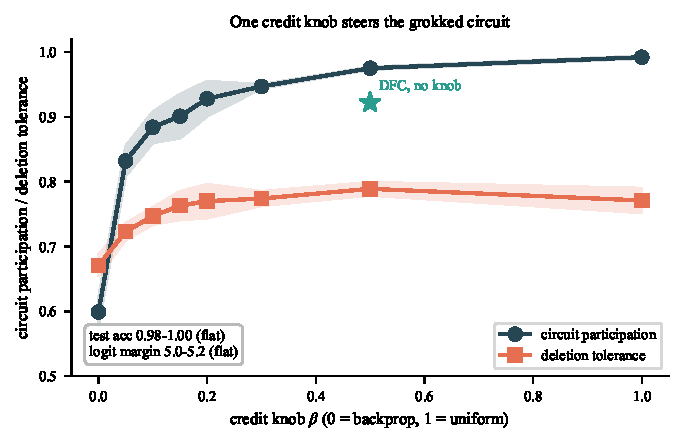
\includegraphics[width=0.62\linewidth]{figures/fig3_steer.pdf}\end{center}
\caption{Turning the knob moves the circuit continuously while nothing else moves. Circuit participation and deletion tolerance against the knob strength $\beta$ on modular addition at $p=31$, three seeds, with test accuracy, logit margin and training loss held across the sweep. The star marks where DFC lands without any knob.}
\label{fig:steer}
\end{figure}

\begin{figure}[!ht]
\begin{center}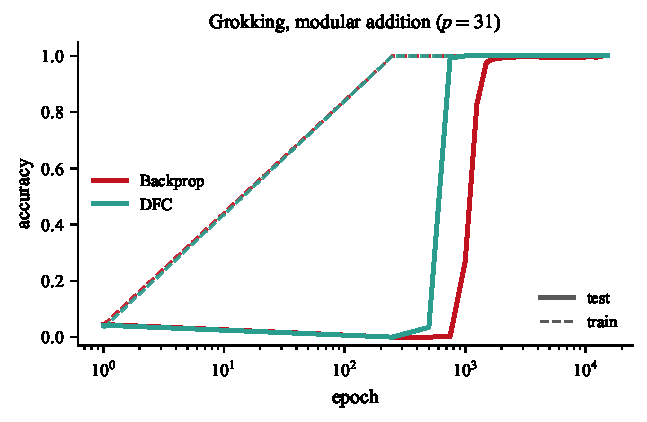
\includegraphics[width=0.52\linewidth]{figures/fig1_grok.pdf}\end{center}
\caption{Backpropagation and DFC grok to perfect test accuracy after a delay. Train and test accuracy over training for both rules on modular addition, same initialization (faint = train, solid = test).}
\label{fig:grok}
\end{figure}

Backpropagation fixes the reference circuit, since it is the rule every published study of the grokked circuit uses, and DFC is the working rule furthest from it. Both show the grokking signature (Figure~\ref{fig:grok}). Training accuracy saturates by epoch $250$ for both, while test accuracy sits at chance for hundreds of epochs more, crossing $0.95$ at epoch $1500$ for backpropagation and $750$ for DFC on this seed.

Three measures show the difference (Figure~\ref{fig:endpoints}). The concentrated and distributed split appears in the input embedding spectra of panel (a) as well as over units. Panel (b) has participation, spectral entropy and per-neuron periodicity rising together, and periodicity matters because a circuit could spread by making every unit respond to many frequencies, which would lower it. It rises instead, so DFC spreads the circuit while each unit tunes to one frequency more sharply.

Panel (c) shows the gap growing with problem size. The number of frequencies DFC needs for $95\%$ accuracy rises from about $10$ at $p=23$ to $18$ at $p=59$, while backpropagation's count stays flat, slope $0.03$ with interval $[-0.12, 0.18]$ and a slope difference of $0.16$ with $95\%$ interval $[0.04, 0.28]$. That is again a difference in the layout and not in the computation both rules perform (Appendix~\ref{app:algo}). We count frequencies by adding them in order of aggregate power until accuracy reaches $95\%$ of its full value, over four seeds at each modulus.

\begin{figure}[!ht]
\begin{center}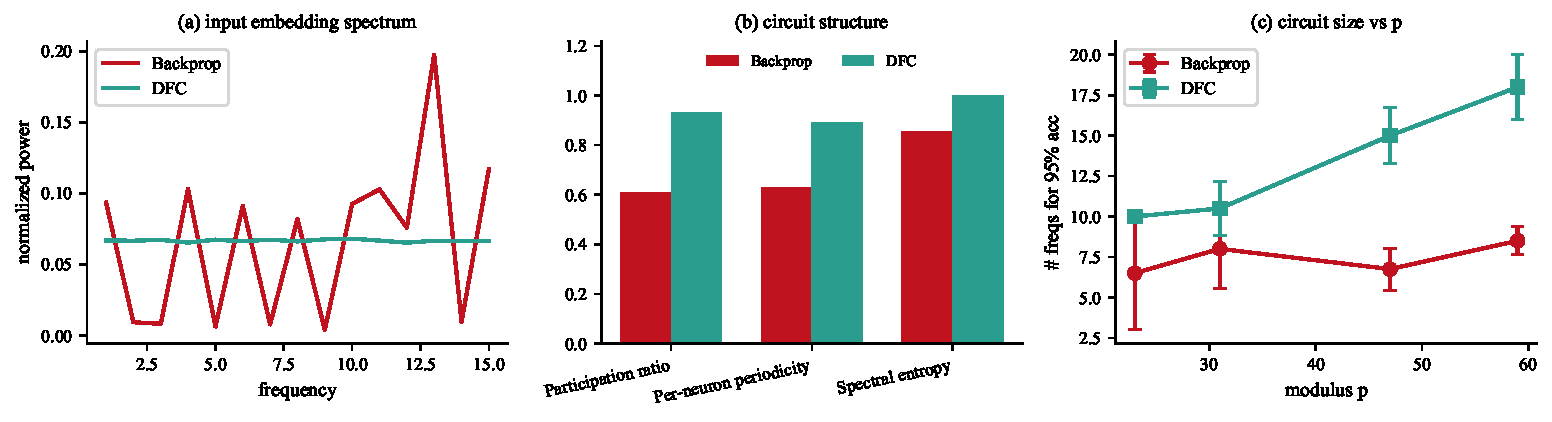
\includegraphics[width=\linewidth]{figures/fig2_endpoints.pdf}\end{center}
\caption{The two rules realize the same algorithm over different numbers of units. (a) input embedding Fourier spectra, sparse peaks for backpropagation versus a flat spectrum for DFC. (b) participation ratio, per-neuron periodicity, and spectral entropy. (c) number of frequencies for $95\%$ accuracy versus $p$, where DFC's count grows faster than backpropagation's (slope difference $0.16$, $95\%$ CI $[0.04, 0.28]$).}
\label{fig:endpoints}
\end{figure}

\begin{figure}[!ht]
\begin{center}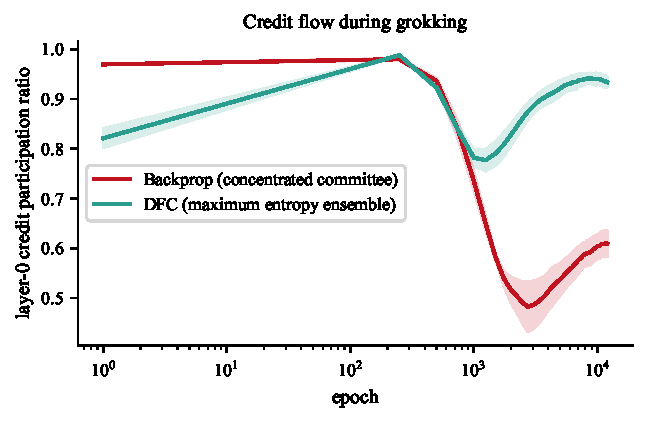
\includegraphics[width=0.55\linewidth]{figures/fig5_creditflow.pdf}\end{center}
\caption{Both rules concentrate credit during the grokking transition, but backpropagation's concentration is deep and persists while DFC's is shallow and transient. Input layer credit participation over training (four seeds, bands are one standard deviation).}
\label{fig:creditflow}
\end{figure}

Credit over training shows the mechanism in time (Figure~\ref{fig:creditflow}, four seeds). Backpropagation's input layer credit PR collapses from near $0.97$ to about $0.48$ and settles near $0.60$, so the concentration stays in the grokked solution, while DFC dips only to about $0.78$ and returns to $0.93$, passing through the transition and coming back distributed. Concentrating credit is therefore part of how grokking happens under both rules, and what tells the rules apart is whether the concentration is released once the circuit is found.

\begin{figure}[!ht]
\begin{center}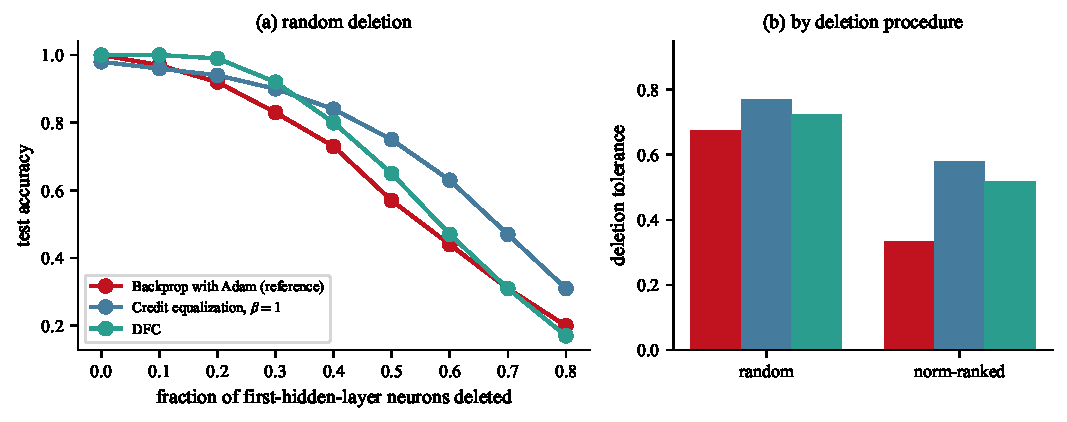
\includegraphics[width=\linewidth]{figures/fig4_fragility.pdf}\end{center}
\caption{Distributed circuits keep far more accuracy under unit deletion, while DFC's fuller frequency ensemble is the most robust to frequency removal. Deletion tolerance for backpropagation, the credit knob at $\beta=1$, and DFC. \textbf{(a)} test accuracy as a fraction of hidden units is randomly dropped. \textbf{(b)} test accuracy as input frequencies are randomly removed. \textbf{(c)} area under the damage curve by attack type. Targeted deletion removes the highest norm units first and magnitude pruning removes the largest weights, both deterministic, so the ordering under those attacks cannot be explained by averaging over random masks.}
\label{fig:fragile}
\end{figure}

Damage separates the two ends (Figure~\ref{fig:fragile}, Table~\ref{tab:dissoc}). Under random unit deletion the distributed circuits rank by participation, the knob gaining $+0.07$, $+0.10$ and $+0.14$ over backpropagation at $p = 23, 31, 59$. Under random frequency removal the ranking reverses, DFC gaining $+0.16$, $+0.16$ and $+0.11$, since only DFC spreads the computation over frequencies as well as units, and each spread protects only against the damage that attacks it. DFC's dropout advantage shrinks with $p$ and is gone at $p = 59$, so robustness follows from how the credit spread the circuit, not from which rule trained it.

Distributed circuits also survive targeted deletions better (Table~\ref{tab:targeted}), the knob at $0.58$ and DFC at $0.52$ against backpropagation's $0.33$ when the highest norm units go first, and pruning the largest input weights first leaves both of them above backpropagation as well. A concentrated circuit depends on exactly the units a targeted attack removes first, so no averaging argument explains the gap.

The gap and its consequence hold on all three operations (Table~\ref{tab:ops}). Multiplication is the sharpest case, where backpropagation lands at participation $0.43$ against the knob's $0.99$, so the effect is largest where backpropagation concentrates hardest (Appendix~\ref{app:scope}).

\begin{table}[!ht]
\caption{Under deterministic attacks the distributed rules' advantage widens, so no averaging argument explains it. Deletion tolerance by damage type at $p=31$ (three seeds). Targeted deletion removes the highest outgoing norm units first, and pruning zeroes the largest input weights first. This is an independent run from Table~\ref{tab:dissoc}, so its random deletion row differs from that table's $p=31$ values.}
\label{tab:targeted}
\begin{center}
\small
\begin{tabular}{lccc}
\toprule
Damage & backprop & knob ($\beta{=}1$) & DFC \\
\midrule
Random unit deletion   & $0.674$ & $\mathbf{0.770}$ & $0.725$ \\
Targeted unit deletion & $0.332$ & $\mathbf{0.581}$ & $0.518$ \\
Magnitude pruning      & $0.237$ & $0.358$ & $\mathbf{0.400}$ \\
\bottomrule
\end{tabular}
\end{center}
\end{table}

\begin{table}[!ht]
\caption{The distributed rules keep more accuracy under every damage type and at every modulus. Deletion tolerance by damage type, rule, and modulus (mean and standard deviation over three seeds). Bold marks the most robust rule per row pair. At $p = 23$ backpropagation and the knob do not fully grok within the budget, which inflates the variances there.}
\label{tab:dissoc}
\begin{center}
\small
\begin{tabular}{llccc}
\toprule
Damage & $p$ & backprop & knob ($\beta{=}1$) & DFC \\
\midrule
Unit dropout      & $23$ & $0.576 \pm 0.038$ & $0.648 \pm 0.055$ & $\mathbf{0.674 \pm 0.022}$ \\
                  & $31$ & $0.671 \pm 0.013$ & $\mathbf{0.767 \pm 0.020}$ & $0.716 \pm 0.011$ \\
                  & $59$ & $0.703 \pm 0.013$ & $\mathbf{0.847 \pm 0.002}$ & $0.699 \pm 0.003$ \\
\midrule
Frequency removal & $23$ & $0.532 \pm 0.044$ & $0.513 \pm 0.044$ & $\mathbf{0.696 \pm 0.022}$ \\
                  & $31$ & $0.622 \pm 0.009$ & $0.652 \pm 0.016$ & $\mathbf{0.783 \pm 0.015}$ \\
                  & $59$ & $0.888 \pm 0.013$ & $0.951 \pm 0.007$ & $\mathbf{0.996 \pm 0.001}$ \\
\bottomrule
\end{tabular}
\end{center}
\end{table}

\begin{table}[!ht]
\caption{The participation gap between the rules, and its deletion consequence, replicate on all three operations. Test accuracy, circuit participation, and deletion tolerance for each rule ($p=31$, three seeds, standard deviations in parentheses, training fraction $0.60$ for addition and $0.58$ for subtraction and multiplication).}
\label{tab:ops}
\begin{center}
\begin{tabular}{llccc}
\toprule
Operation & Rule & Test & Circuit PR & Random del \\
\midrule
Addition       & backprop & $0.998\,(0.001)$ & $0.60\,(0.02)$ & $0.671\,(0.016)$ \\
               & knob ($\beta{=}1$) & $0.976\,(0.011)$ & $0.99\,(0.00)$ & $0.771\,(0.019)$ \\
               & DFC & $1.000\,(0.000)$ & $0.92\,(0.00)$ & $0.717\,(0.014)$ \\
\midrule
Subtraction    & backprop & $0.999\,(0.001)$ & $0.59\,(0.04)$ & $0.680\,(0.026)$ \\
               & knob ($\beta{=}1$) & $0.994\,(0.005)$ & $0.99\,(0.00)$ & $0.785\,(0.014)$ \\
               & DFC & $1.000\,(0.000)$ & $0.93\,(0.01)$ & $0.735\,(0.010)$ \\
\midrule
Multiplication & backprop & $0.999\,(0.001)$ & $0.43\,(0.07)$ & $0.666\,(0.035)$ \\
               & knob ($\beta{=}1$) & $0.999\,(0.001)$ & $0.99\,(0.00)$ & $0.867\,(0.012)$ \\
               & DFC & $1.000\,(0.000)$ & $0.86\,(0.02)$ & $0.764\,(0.010)$ \\
\bottomrule
\end{tabular}
\end{center}
\end{table}

\section{Long run stability and rule switching}
\label{app:long}
If the concentrated circuit were a stop on the way rather than a destination, backpropagation would drift toward the distributed one given a long enough run, and the knob would only be a shortcut. That reading has theory behind it, since the knob's solution is the one max-margin theory calls asymptotically optimal \citep{morwani2024feature} and it sits at backpropagation's own margin normalized norm (Appendix~\ref{app:norm}).

Backpropagation does not drift. Trained for $200{,}000$ epochs, ten times the budget used anywhere else in the paper, its participation settles by roughly $40{,}000$ epochs and is then constant to three decimals, ending at $0.605\,(0.012)$ against the knob's $0.990\,(0.003)$ (Table~\ref{tab:long}). The concentrated circuit is the solution backpropagation occupies, not a waypoint, so selection is the correct description.

The same run shows when credit and circuit come to agree. Both start near uniform, since at initialization every unit receives comparable credit, then fall together through the grokking transition and settle together, staying within about $0.06$ of each other at every checkpoint. Credit participation describes the solution a rule is building as it builds it, which is why we call the agreement a correspondence.

A circuit stable under the rule that built it could still be stable in two ways: in itself, inherited from the grokking transition, or held in place by the rule. A switch separates them, since an inherited circuit would stay put whatever rule runs afterwards and a maintained one should move. We grok at one setting for $20{,}000$ epochs, continue for $30{,}000$ at the other, and run both same rule continuations as drift controls (Table~\ref{tab:long}).

The circuit is maintained. Turning the knob on after backpropagation has grokked moves participation from $0.613\,(0.016)$ to $0.991\,(0.000)$ within the first $5000$ epochs, at test accuracy $0.997$ throughout, while the backpropagation control holds at $0.610\,(0.012)$, so the reorganization is the rule and not the extra training. Removing the knob re-concentrates the distributed circuit to $0.722\,(0.016)$, still falling at the end of the phase, while its control holds at $0.990\,(0.003)$. Both networks had finished the task before the switch and stay at the ceiling through it, so nothing is being learned: the same function is rebuilt over a different set of units because a different rule now assigns the credit. Together with the long run, a rule holds its own circuit indefinitely and moves the other rule's circuit when applied to it.

\begin{table}[!ht]
\caption{The two ends are different solutions rather than one reached at two speeds, and each rule holds its own circuit indefinitely while moving the other rule's circuit when applied to it. Long run stability and rule switching ($p=31$, three seeds, standard deviations in parentheses). In the held block the rule never changes and the two circuit columns are participation at $20{,}000$ and at $200{,}000$ epochs, ten times the budget used anywhere else, with backpropagation's participation constant from about $40{,}000$ epochs onward. In the switched block phase one runs $20{,}000$ epochs and phase two a further $30{,}000$ at the setting named, so the two circuit columns are participation after each phase, and the same rule rows are the drift controls. Credit is the applied per-unit credit participation during phase two, which confirms each phase applied the rule it names, and targeted deletion was measured only on the held runs.}
\label{tab:long}
\begin{center}
\footnotesize
\setlength{\tabcolsep}{4pt}
\begin{tabular}{lcccccc}
\toprule
Condition & Circuit before & Circuit after & Credit & Test & Random del & Targeted del \\
\midrule
\multicolumn{7}{l}{\emph{Rule held, $20{,}000$ to $200{,}000$ epochs}} \\
Backpropagation ($\beta{=}0$) & $0.60$ & $0.605\,(0.012)$ & --- & $0.997$ & $0.673$ & $0.298$ \\
Equalized ($\beta{=}1$) & $0.99$ & $0.990\,(0.003)$ & --- & $0.975$ & $0.775$ & $0.599$ \\
\midrule
\multicolumn{7}{l}{\emph{Rule switched, phase one to phase two}} \\
$\beta{=}0 \to \beta{=}1$ & $0.613\,(0.016)$ & $0.991\,(0.000)$ & $0.999$ & $0.997$ & $0.800$ & --- \\
$\beta{=}1 \to \beta{=}0$ & $0.990\,(0.003)$ & $0.722\,(0.016)$ & $0.719$ & $0.990$ & $0.703$ & --- \\
$\beta{=}0 \to \beta{=}0$ & $0.613\,(0.016)$ & $0.610\,(0.012)$ & $0.601$ & $0.997$ & $0.675$ & --- \\
$\beta{=}1 \to \beta{=}1$ & $0.990\,(0.003)$ & $0.990\,(0.003)$ & $1.000$ & $0.975$ & $0.775$ & --- \\
\bottomrule
\end{tabular}
\end{center}
\end{table}

\section{Adaptation to a new operation}
\label{app:adapt}
This appendix measures adaptation speed, the training time to reach a new task from each grokked circuit. We grok on modular addition at $p=31$ at each setting of $\beta$, then fine-tune the whole network on a second operation with plain backpropagation, identically in every condition, counting epochs until test accuracy reaches $0.9$ (Table~\ref{tab:adapt}).

\begin{table}[!ht]
\caption{Full fine-tuning from a grokked circuit to a new operation, five or more seeds per condition, standard deviations in parentheses. Epochs count until test accuracy $0.9$ on the new operation. Free units are those whose outgoing norm falls below a tenth of the mean.}
\label{tab:adapt}
\begin{center}
\small
\begin{tabular}{lcccccc}
\toprule
Condition & Circuit PR & Free units & Source test & \multicolumn{2}{c}{Epochs to $0.9$} \\
 & & & & to sub & to mul \\
\midrule
$\beta=0$ (backprop) & $0.593\,(0.034)$ & $85$ & $0.995$ & $640\,(128)$  & $1800\,(141)$ \\
$\beta=0.25$         & $0.933\,(0.020)$ & $0$  & $0.989$ & $940\,(191)$  & $1940\,(233)$ \\
$\beta=0.5$          & $0.972\,(0.006)$ & $0$  & $0.990$ & $1200\,(89)$  & $1980\,(248)$ \\
$\beta=0.75$         & $0.983\,(0.003)$ & $0$  & $0.981$ & $1300\,(141)$ & $2020\,(133)$ \\
$\beta=1$            & $0.991\,(0.002)$ & $0$  & $0.972$ & $1540\,(180)$ & $1940\,(136)$ \\
From scratch         & ---              & ---  & ---     & $1410\,(137)$ & $1200\,(63)$ \\
\bottomrule
\end{tabular}
\end{center}
\end{table}

Adaptation to subtraction slows monotonically with the starting circuit's spread, at a rank correlation of $+1.00$ with participation, and the two ends do not overlap: every backpropagation seed lands between $400$ and $800$ epochs, every equalized seed between $1200$ and $1800$.

The free unit column separates two mechanisms. Backpropagation leaves about $85$ units carrying almost nothing, which a new task can claim instead of disturbing working structure. That count is already zero at $\beta=0.25$, yet adaptation keeps slowing all the way to $1540$ at $\beta=1$. Spare capacity therefore explains the jump from backpropagation to the distributed settings, and the continued rise among them means that the more evenly the work is spread, the more of it a new task has to disturb.

Multiplication is a different regime: every pretrained condition is slower than a fresh initialization, $1800$ to $2020$ epochs against $1200$, so what addition built gets in the way. The trade-off is therefore a claim about targets that benefit from the source task, which subtraction does and multiplication does not.

The direction is not special either. Subtraction to addition reproduces the effect, $740$ epochs at $\beta=0$ rising to $1600$ at $\beta=1$, again monotone at a rank correlation of $+1.00$.

Freezing the hidden circuit and retraining only the readout does not work at all: every condition stays at chance, at test $0.012$ or below. The units are not a reusable basis but combinations built for one operation, since units trained on $a+b$ compute quantities such as $\cos(\theta_a + \theta_b - \phi)$, and no linear combination of those gives the $\cos(\theta_a - \theta_b)$ that subtraction needs.

\section{Generality and boundaries}
The paper's headline results are modular arithmetic in a multilayer perceptron. This section tests how far the result reaches and reports where it stops as carefully as where it holds. One statement with a condition covers everything below: the knob spreads a circuit wherever the gradient left a concentration, and it does nothing where the gradient did not.

\subsection{All settings of the knob}
\label{app:scope}
\begin{table}[!ht]
\caption{The knob moves the circuit wherever a concentration exists to move. Every setting we applied it in, as circuit participation at $\beta{=}0$ and $\beta{=}1$. Test accuracy is within a point of backpropagation's in every row except addition, where full equalization costs about two points. The last three rows are boundaries rather than failures, since no concentration is left for the knob to act on.}
\label{tab:scope}
\begin{center}
\footnotesize
\setlength{\tabcolsep}{5pt}
\begin{tabular}{llccl}
\toprule
Setting & Circuit measured & $\beta{=}0$ & $\beta{=}1$ & Evidence \\
\midrule
Addition, subtraction, multiplication & hidden units & $0.43$--$0.60$ & $0.99$ & Table~\ref{tab:ops} \\
Sparse parity           & hidden units & $0.15$ & $0.96$ & App.~\ref{app:parity} \\
$S_5$, non-abelian      & hidden units & $0.70$ & $0.97$ & App.~\ref{app:groups} \\
Transformer, $p=31$, wide MLP & MLP block & $0.61$ & $0.99$ & App.~\ref{app:transformer} \\
\midrule
Transformer, $p=113$ canonical & MLP block & $0.96$ & $0.96$ & App.~\ref{app:transformer} \\
Transformer, two blocks & MLP block & $0.85$ & $0.88$ & App.~\ref{app:transformer} \\
MNIST                   & hidden units & $0.99$ & $0.99$ & App.~\ref{app:mnist} \\
\bottomrule
\end{tabular}
\end{center}
\end{table}

\subsection{The endpoint gap across widths and depths}
\label{app:arch}
The endpoint gap does not depend on the particular network. At widths $256$ and $512$ and depths two and three, backpropagation stays concentrated and DFC stays distributed (Table~\ref{tab:arch}), with DFC's spectral entropy at essentially $1.0$ throughout.

Doubling the width needs care, because participation is a \emph{fraction} of the layer. Backpropagation's fraction falls from $0.61$ to $0.40$, which looks more concentrated, while its effective unit count rises from $156$ to $205$, which looks less. Both are correct, they answer different questions, and neither touches the paper's comparison, since DFC is above backpropagation at every width and depth on both. Deciding which better describes the concentrated endpoint would take a width sweep, so we leave it open.

The gap is also not an artifact of idle units. Restricted to units above the free unit threshold, an outgoing norm of at least a tenth of the mean, backpropagation's working units sit at participation $0.889\,(0.006)$ with $84$ idle, the knob's at $0.991\,(0.001)$ with none, and $\beta=0.25$ reaches $0.935$ with none idle either (three seeds). The knob both stops units going idle and evens out the ones that work.

\begin{table}[!ht]
\caption{Backpropagation stays concentrated and DFC stays distributed at every width and depth. Circuit across architectures (modular addition, $p=31$, three seeds). Participation is normalized by width, so $n \cdot \mathrm{PR}$ is given beside it: backpropagation's fraction falls with width while its effective unit count rises.}
\label{tab:arch}
\begin{center}
\begin{tabular}{lcccccc}
\toprule
 & \multicolumn{2}{c}{Participation ratio} & \multicolumn{2}{c}{Effective units $n \cdot \mathrm{PR}$}
 & \multicolumn{2}{c}{Per-neuron periodicity} \\
\cmidrule(lr){2-3}\cmidrule(lr){4-5}\cmidrule(lr){6-7}
Architecture & Backprop & DFC & Backprop & DFC & Backprop & DFC \\
\midrule
width 256, depth 2 & $0.61$ & $0.93$ & $156$ & $238$ & $0.63$ & $0.89$ \\
width 512, depth 2 & $0.40$ & $0.82$ & $205$ & $420$ & $0.53$ & $0.82$ \\
width 256, depth 3 & $0.52$ & $0.87$ & $133$ & $223$ & $0.57$ & $0.87$ \\
\bottomrule
\end{tabular}
\end{center}
\end{table}

\subsection{Sparse parity}
\label{app:parity}
This is the one task in the paper where DFC fails, and that is why we ran it. Everywhere else the distributed end can be reached two ways, by the controller or by the knob, so one can ask whether the mechanism comes from the credit distribution or from DFC in particular, and here only the knob works.

The task is $(20, 3)$ sparse parity: the label is the parity of a fixed set of three of the $20$ input bits, and the rest are distractors. We run two dataset sizes, roughly $2000$ and $300$ training examples. Two things make it a boundary. In our full batch regime every rule that solves it generalizes without a grokking delay, so parity is not a grokking testbed here. And DFC does not solve it: test accuracy stalls between $0.82$ and $0.92$ across seeds and sizes, so its inductive bias suits modular structure rather than parity.

The knob works exactly as on the modular tasks, reaching participation $0.89$ to $0.96$ against backpropagation's $0.08$ to $0.15$, with markedly better dropout robustness at both sizes (Table~\ref{tab:parity}), so the chain from credit to robustness holds where DFC does not and the mechanism is a property of the credit distribution and not of that rule. One measure does not follow: under uniform weight noise backpropagation is the most robust, since spreading over units helps against losing units, not against perturbing all of them.

\begin{table}[!ht]
\caption{The credit knob works where DFC cannot, so the effect does not depend on the controller. Sparse parity at two dataset sizes (three seeds, standard deviations in parentheses). Backpropagation and the knob both grok to test $1.0$, while DFC does not solve parity, so its rows are the underfit case.}
\label{tab:parity}
\begin{center}
\small
\begin{tabular}{llcccc}
\toprule
Train size & Rule & Test & Circuit PR & Random del & Noise tol \\
\midrule
$\sim 2000$ & backprop & $1.000\,(0.000)$ & $0.15\,(0.06)$ & $0.865\,(0.051)$ & $1.000\,(0.000)$ \\
            & knob ($\beta{=}1$) & $1.000\,(0.000)$ & $0.96\,(0.03)$ & $0.955\,(0.002)$ & $0.988\,(0.016)$ \\
            & DFC & $0.924\,(0.039)$ & $0.04\,(0.01)$ & $0.679\,(0.011)$ & $0.785\,(0.008)$ \\
\midrule
$\sim 300$  & backprop & $1.000\,(0.000)$ & $0.08\,(0.02)$ & $0.825\,(0.017)$ & $0.999\,(0.001)$ \\
            & knob ($\beta{=}1$) & $0.988\,(0.017)$ & $0.89\,(0.02)$ & $0.908\,(0.060)$ & $0.917\,(0.074)$ \\
            & DFC & $0.822\,(0.045)$ & $0.04\,(0.00)$ & $0.648\,(0.005)$ & $0.736\,(0.025)$ \\
\bottomrule
\end{tabular}
\end{center}
\end{table}

\subsection{Composition in \texorpdfstring{$S_5$}{S5}}
\label{app:groups}
Modular addition wraps around, so a network can solve it with a few repeating waves, and every headline result is on a task of that kind, leaving open whether the credit effect is really about that periodic structure. Composing permutations of five objects has no such structure: the solutions are built from the group's irreducible representations rather than frequencies \citep{chughtai2023toy}, so none of our Fourier measures applies and participation, which depends on no basis, carries the analysis. We train the same network on the $120 \times 120$ composition table with one hot inputs, holding out half the pairs. It groks here too, on the same thresholds as modular addition, with the delay lengthening as data is removed (Table~\ref{tab:groups}).

The correspondence survives the move. Each rule's circuit tracks the credit it applies, backpropagation at $0.699\,(0.078)$ from credit $0.689$ and the knob at $0.973\,(0.005)$ from $1.00$, both at test $1.000$. The damage gap is sharper than in the abelian case, targeted deletion leaving backpropagation at $0.149$ against the knob's $0.468$, a factor of three where modular addition gives about $1.8$, and a smaller training fraction reproduces both. DFC underfits here as on parity, so its row carries no structural claim.

\begin{table}[!ht]
\caption{The credit statistic still tracks the circuit on a task with no Fourier structure. Composition in $S_5$ (ten seeds at half the pairs held out, five at $60\%$, standard deviations in parentheses). The concentrated circuit is the least damage tolerant under random and targeted deletion alike, and the grokking delay lengthens as data is removed.}
\label{tab:groups}
\begin{center}
\small
\begin{tabular}{lcccccc}
\toprule
Rule & Test & Credit PR & Circuit PR & Random del & Targeted del & Delay \\
\midrule
\multicolumn{7}{l}{\emph{Half the pairs held out, ten seeds}} \\
Backpropagation & $1.000$ & $0.689$ & $0.699\,(0.078)$ & $0.485$ & $0.149$ & $500$ \\
Knob $\beta{=}0.5$ & $1.000$ & $0.970$ & $0.942\,(0.010)$ & $0.585$ & $0.322$ & $550$ \\
Knob $\beta{=}1.0$ & $1.000$ & $1.000$ & $0.973\,(0.005)$ & $0.633$ & $0.468$ & $900$ \\
\midrule
\multicolumn{7}{l}{\emph{$60\%$ held out, less data, five seeds}} \\
Backpropagation & $1.000$ & $0.657$ & $0.662\,(0.038)$ & $0.409$ & $0.129$ & $1350$ \\
Knob $\beta{=}0.5$ & $1.000$ & $0.951$ & $0.907\,(0.016)$ & $0.525$ & $0.260$ & $1650$ \\
Knob $\beta{=}1.0$ & $1.000$ & $1.000$ & $0.970\,(0.002)$ & $0.597$ & $0.410$ & $1750$ \\
\midrule
DFC (underfits) & $0.000$ & $0.853$ & $0.968\,(0.004)$ & --- & --- & --- \\
\bottomrule
\end{tabular}
\end{center}
\end{table}

\subsection{Transformers}
\label{app:transformer}
A transformer gives the knob a choice the multilayer perceptron never did: computation can concentrate in the embedding that reads the tokens or in the multilayer perceptron block that processes them.

The architecture is the standard grokking transformer of the interpretability literature. Modular addition is presented as the sequence ``$a\ b\ =$'', with token and positional embeddings, one attention head per $32$ channels, a ReLU multilayer perceptron block of width $4d_{\text{model}}$, and weight decay $1.0$. Its canonical configuration is one block at $p=113$ with $d_{\text{model}}=128$.

Trained with backpropagation it groks to test accuracy $1.0$, and its two components land on opposite sides: the block is already \emph{distributed} at participation $0.96$, and the token embedding is \emph{concentrated}, its Fourier power carried by $21$ of the $56$ available frequencies. The split is a matter of spare capacity, since concentrating means leaving units idle and this block has no room for that.

The knob therefore acts on the embedding, and equalizing credit across every linear map raises every embedding and block measure monotonically across three settings of $\beta$, at test $1.000$ throughout and at a second modulus and twice the width as well (Table~\ref{tab:transformer}). Applying the knob to the block alone does nothing, as it should.

Give the block the room instead and the concentration moves into it. A $4096$ unit block at $p=31$ leaves capacity idle, and participation runs from $0.610\,(0.048)$ to $0.993\,(0.003)$ over five seeds with no overlap, targeted deletion tolerance following from $0.580$ to $0.941$ at unchanged accuracy and margin. Spare capacity, not training time, creates the opportunity: at $p=23$ the block sits near $0.90$ and does not concentrate, and running $100$k epochs instead of $30$k changes nothing.

Width sets how much room the knob has without saying where concentration appears, and here one of our predictions failed: sweeping the block from $256$ to $4096$ units, the knob's gain rises monotonically with width as expected, $0.047$ through $0.402$, but the baseline it acts on falls unevenly, which we did not expect. The paper's result is the five seed confirmation above, not the sweep's shape.

Two blocks give a third case of the condition. The baseline settles already distributed, at $0.851\,(0.029)$ over ten seeds, so there is little to redistribute. The knob still moves participation to $0.878\,(0.032)$ and deletion tolerance from $0.430$ to $0.546$, and we read this as the condition holding, not as support for the effect.

\begin{table}[!ht]
\caption{The knob acts on whatever component holds the concentration, which in a one-block transformer is the embedding, since its multilayer perceptron block is already distributed. Transformers on modular addition (standard deviations in parentheses, $\beta{=}0$ is plain backpropagation). Frequencies is the number of embedding frequencies holding $95\%$ of the non-DC power. Test accuracy is $1.000$ in every row, and the two block runs are reported in the text, since they do not log the embedding measures.}
\label{tab:transformer}
\begin{center}
\footnotesize
\setlength{\tabcolsep}{4pt}
\begin{tabular}{lcccccc}
\toprule
$\beta$ & Test & MLP part. & Embed entropy & Freqs & MLP random del & Embed freq del \\
\midrule
\multicolumn{7}{l}{\emph{Canonical: one block, $p=113$, $d_{\text{model}}=128$, all layers knob, six seeds}} \\
$0.0$ & $1.000$ & $0.955\,(0.01)$ & $0.776\,(0.02)$ & $21.0\,(2.3)$ & $0.817\,(0.07)$ & $0.852\,(0.03)$ \\
$0.5$ & $1.000$ & $0.953\,(0.01)$ & $0.800\,(0.01)$ & $23.5\,(1.3)$ & $0.857\,(0.04)$ & $0.864\,(0.03)$ \\
$1.0$ & $1.000$ & $0.955\,(0.01)$ & $0.823\,(0.01)$ & $26.0\,(1.3)$ & $0.900\,(0.02)$ & $0.878\,(0.02)$ \\
\midrule
\multicolumn{7}{l}{\emph{Second modulus: $p=97$, three seeds, $70$k epochs}} \\
$0.0$ & $1.000$ & $0.959\,(0.01)$ & $0.814\,(0.00)$ & $21.3\,(0.5)$ & $0.854\,(0.02)$ & $0.810\,(0.01)$ \\
$1.0$ & $1.000$ & $0.951\,(0.02)$ & $0.864\,(0.02)$ & $26.3\,(2.1)$ & $0.909\,(0.03)$ & $0.841\,(0.04)$ \\
\midrule
\multicolumn{7}{l}{\emph{Twice the width: $d_{\text{model}}=256$, three seeds}} \\
$0.0$ & $1.000$ & $0.902\,(0.04)$ & $0.821\,(0.01)$ & $25.0\,(2.2)$ & $0.950\,(0.01)$ & $0.935\,(0.01)$ \\
$1.0$ & $1.000$ & $0.917\,(0.01)$ & $0.861\,(0.01)$ & $29.3\,(1.7)$ & $0.969\,(0.01)$ & $0.954\,(0.01)$ \\
\bottomrule
\end{tabular}
\end{center}
\end{table}

\subsection{MNIST}
\label{app:mnist}
The knob needs a concentrated solution to act on, and MNIST does not have one. We run the setting in which grokking on real images has been reported \citep{liu2022omnigrok}, a training subset of $1000$ images and a two hidden layer network of width $200$, at the standard and a large initialization scale.

Two things happen. Training and test accuracy rise together with no delay, so we are not measuring a grokked circuit. And backpropagation's credit is already nearly uniform, at participation $0.932$ against $0.59$ on modular addition, with the circuit distributed to match at $0.992\,(0.002)$. The knob has almost nothing to redistribute, and at $\beta=1$ nothing changes within noise.

Nothing moving is the correct outcome, not a failure. Credit that is already near uniform predicts a circuit that is already distributed, so MNIST bounds when the credit effect is informative, not whether it is real. The low dimensional solutions and one hot inputs of modular arithmetic and group composition concentrate the gradient on a few directions, and a dense image task does not.

\end{document}

